\documentclass[12pt]{article}
\usepackage[left=1.15in, right=1.15in, top=1in, bottom=1.5in]{geometry}
\usepackage{natbib}
\usepackage{verbatim}
\usepackage{setspace}
\usepackage{booktabs}
\usepackage{caption}
\usepackage{graphicx}
\usepackage{subcaption}
\bibpunct[: ]{(}{)}{;}{a}{}{,} 
\usepackage{authblk}
\renewcommand\Authfont{\normalsize}
\renewcommand\Affilfont{\footnotesize}

\begin{document}
\title{The Forward March of Categorical Tolerance in the United States\thanks{Reserved for acknowledgments}}
\author[1]{Omar Lizardo\thanks{olizardo@soc.ucla.edu}}
\affil[1]{Department of Sociology, UCLA}

\renewcommand\Authands{ and }

\date{\normalsize \today}	
\maketitle

\newpage
\begin{abstract}
\end{abstract}
\newpage
\section*{Introduction}
In a paper published almost a decade ago, \citet{lizardo2016end-4fb}---hereafter L\&S---introduced the idea of \textit{categorical tolerance} to refer to the phenomenon of a growing proportion of the population who refuse to report dislikes of \textit{any} cultural genres---typically musical genres---in a standard social science survey design to measure patterns of cultural taste. In that paper, L\&S noted that categorical tolerance appeared to be on the rise in the United States, going from about five percent of the population in the classic 1993 General Social Survey culture module to about sixteen percent in a then-recent survey of a representative sample of Americans collected in 2012, which matched the GSS 1993 battery of items on likes and dislikes of musical tastes across eighten genres. This resulted in a significant shift in the shape of the univariate count distributions of number of dislikes, which went from a standard Poisson distribution in the GSS 1993 to a count distribution with excess zeroes in 2012 \citep[p.90, Figure 1]{lizardo2016end-4fb}. 

In that paper, L\&S also showed that the rise of categorical tolerance among Americans was a socially patterned phenomenon. Particularly, L\&S showed that refusal to dislike was a growing trend among more recently born cohorts, suggestive of a macro-level pattern of cultural change via cohort replacement of the type that has been more recently shown to govern cultural change across a wide variety of values, attitudes, beliefs, and practices \citep{vaisey2016cultural-867, kiley2020measuring-123, keskintrk2025what-483, vaisey2021model-based-deb}. In the same way, comparison of 2012 and 1993 data suggested that categorical tolerants were over-represented among non-whites, with a slight under-representation of people with a college degree, indicating that categorical tolerance did not seem to be driven by the usual status and cultural-capital-based dynamics emphasized by Bourdieusian models of social distinction \citep{bourdieu1984distinction-835}, which usually focuses on status display among those with higher education \citep{jarness2017im-001}.

This paper uses recently collected data from a representative sample of the American population to update the empirical picture of categorical tolerance in the United States. First, I ask whether we can observe a continued rise in the categorical tolerance effect in the more recent data. Secondly, I examine the socio-demographic correlates of categorical tolerance to determine whether this pattern of cultural choice persists in a similar socio-demographic niche as L\&S observed in 2012, or whether its location in social space has evolved since then \citep{mcpherson2004blau-9fe}. Third, I also examine the socio-demographic correlates of \textit{symbolic exclusion} among people who express dislikes \citep{bryson1996anything-311}, to see if we can observe similar patterns to those previously uncovered by L\&S. Finally, the paper adds a missing dimension to previous work on categorical tolerance and symbolic exclusion by investigating whether these cultural taste patterns are connected to political identification as liberal or conservative, given recent work indicating that cultural taste patterns have themselves become embroiled in the ``oil spill'' produced by the continuing political polarization of the American mass publics in the last two decades, a phenomenon that has accelerated in the Trump era \citep{dellaposta2020pluralistic-ed4, rawlings2023polarization-0af}.

To preview the main results: I find that, indeed, categorical tolerance has continued its onward march among Americans, with about twenty percent of respondents failing to report disliking any of the twelve genres included in the survey. Secondly, the social location of categorical tolerance is fairly similar to that observed by L\&S a decade ago; younger adults are over-represented among categorical tolerants relative to older adults (and very young respondents). In the same way, just like L\&S found in 2012, non-whites are over-represented among categorical tolerants (excepting Black respondents). Finally, categorical tolerance is not polarized along liberal/conservative lines, but symbolic exclusion is; net of other factors, conservatives are more likely to express a larger number of cultural dislikes than liberals (as are older individuals relative to the young). 

The rest of the paper is organized as follows. The next section briefly reviews recent work that builds on L\&S's idea of categorical tolerance, as well as other work looking at the increasing linkages between cultural taste and political ideology. The next sections introduce the data and outline the basic analytic plan, presenting the main results. Finally, the discussion section summarizes the key findings, highlights their main implications, and suggests avenues for future work. 

\section*{Previous Work}

\section*{Results}
\subsection*{Probability of Dislikes by Genre}
Table~\ref{tab:dis-by-genres} shows the probability of any genre experiencing a judgment of dislike. As we can see, Metal is the genre more likely to be disliked, consistent with previous work in the United States \citep{bryson1996anything-311, lizardo2015musical-8c6}. Electronic Dance Music, Rap/Hip Hop, and Broadway/Musicals are also toward the top in terms of dislikes. R\&B, Rock, and Pop/Top 40, on the other hand, have comparatively low odds of being disliked. 

\subsection*{Univariate Distribution of Number of Dislikes}
\begin{figure}[ht!]
        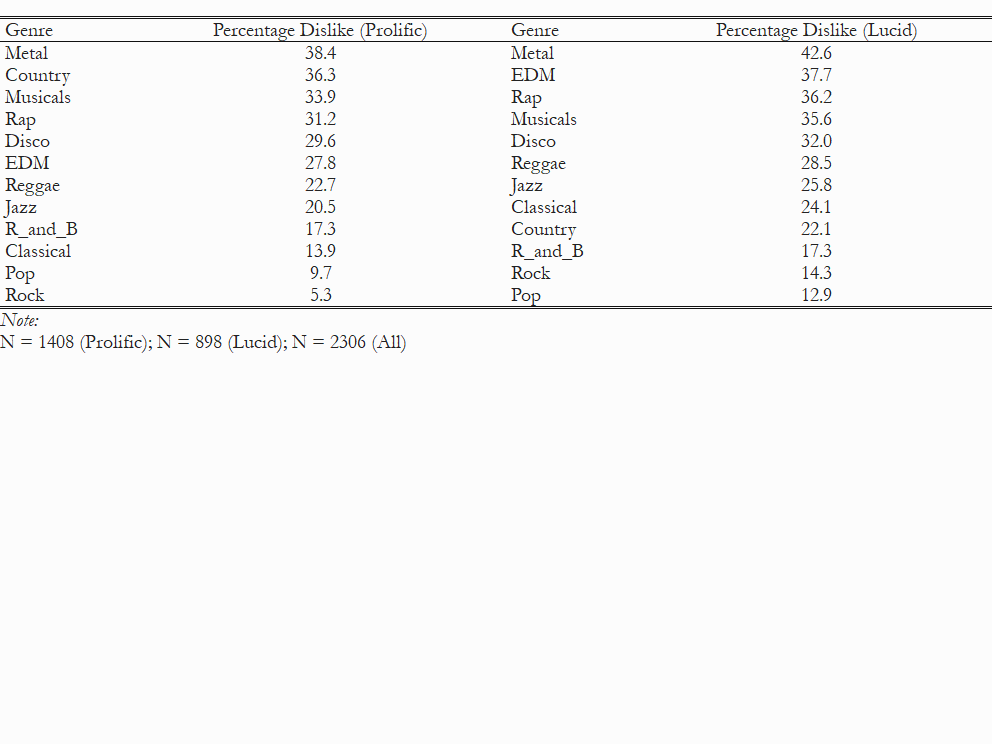
\includegraphics[trim={0 11cm 0 0},clip, width=1.0\textwidth]{Tabs/desc-tab-dislike.png}
    \caption{Proportion of dislikes by genre.}
    \label{tab:dis-by-genres}
\end{figure}

\begin{figure}[ht!]
        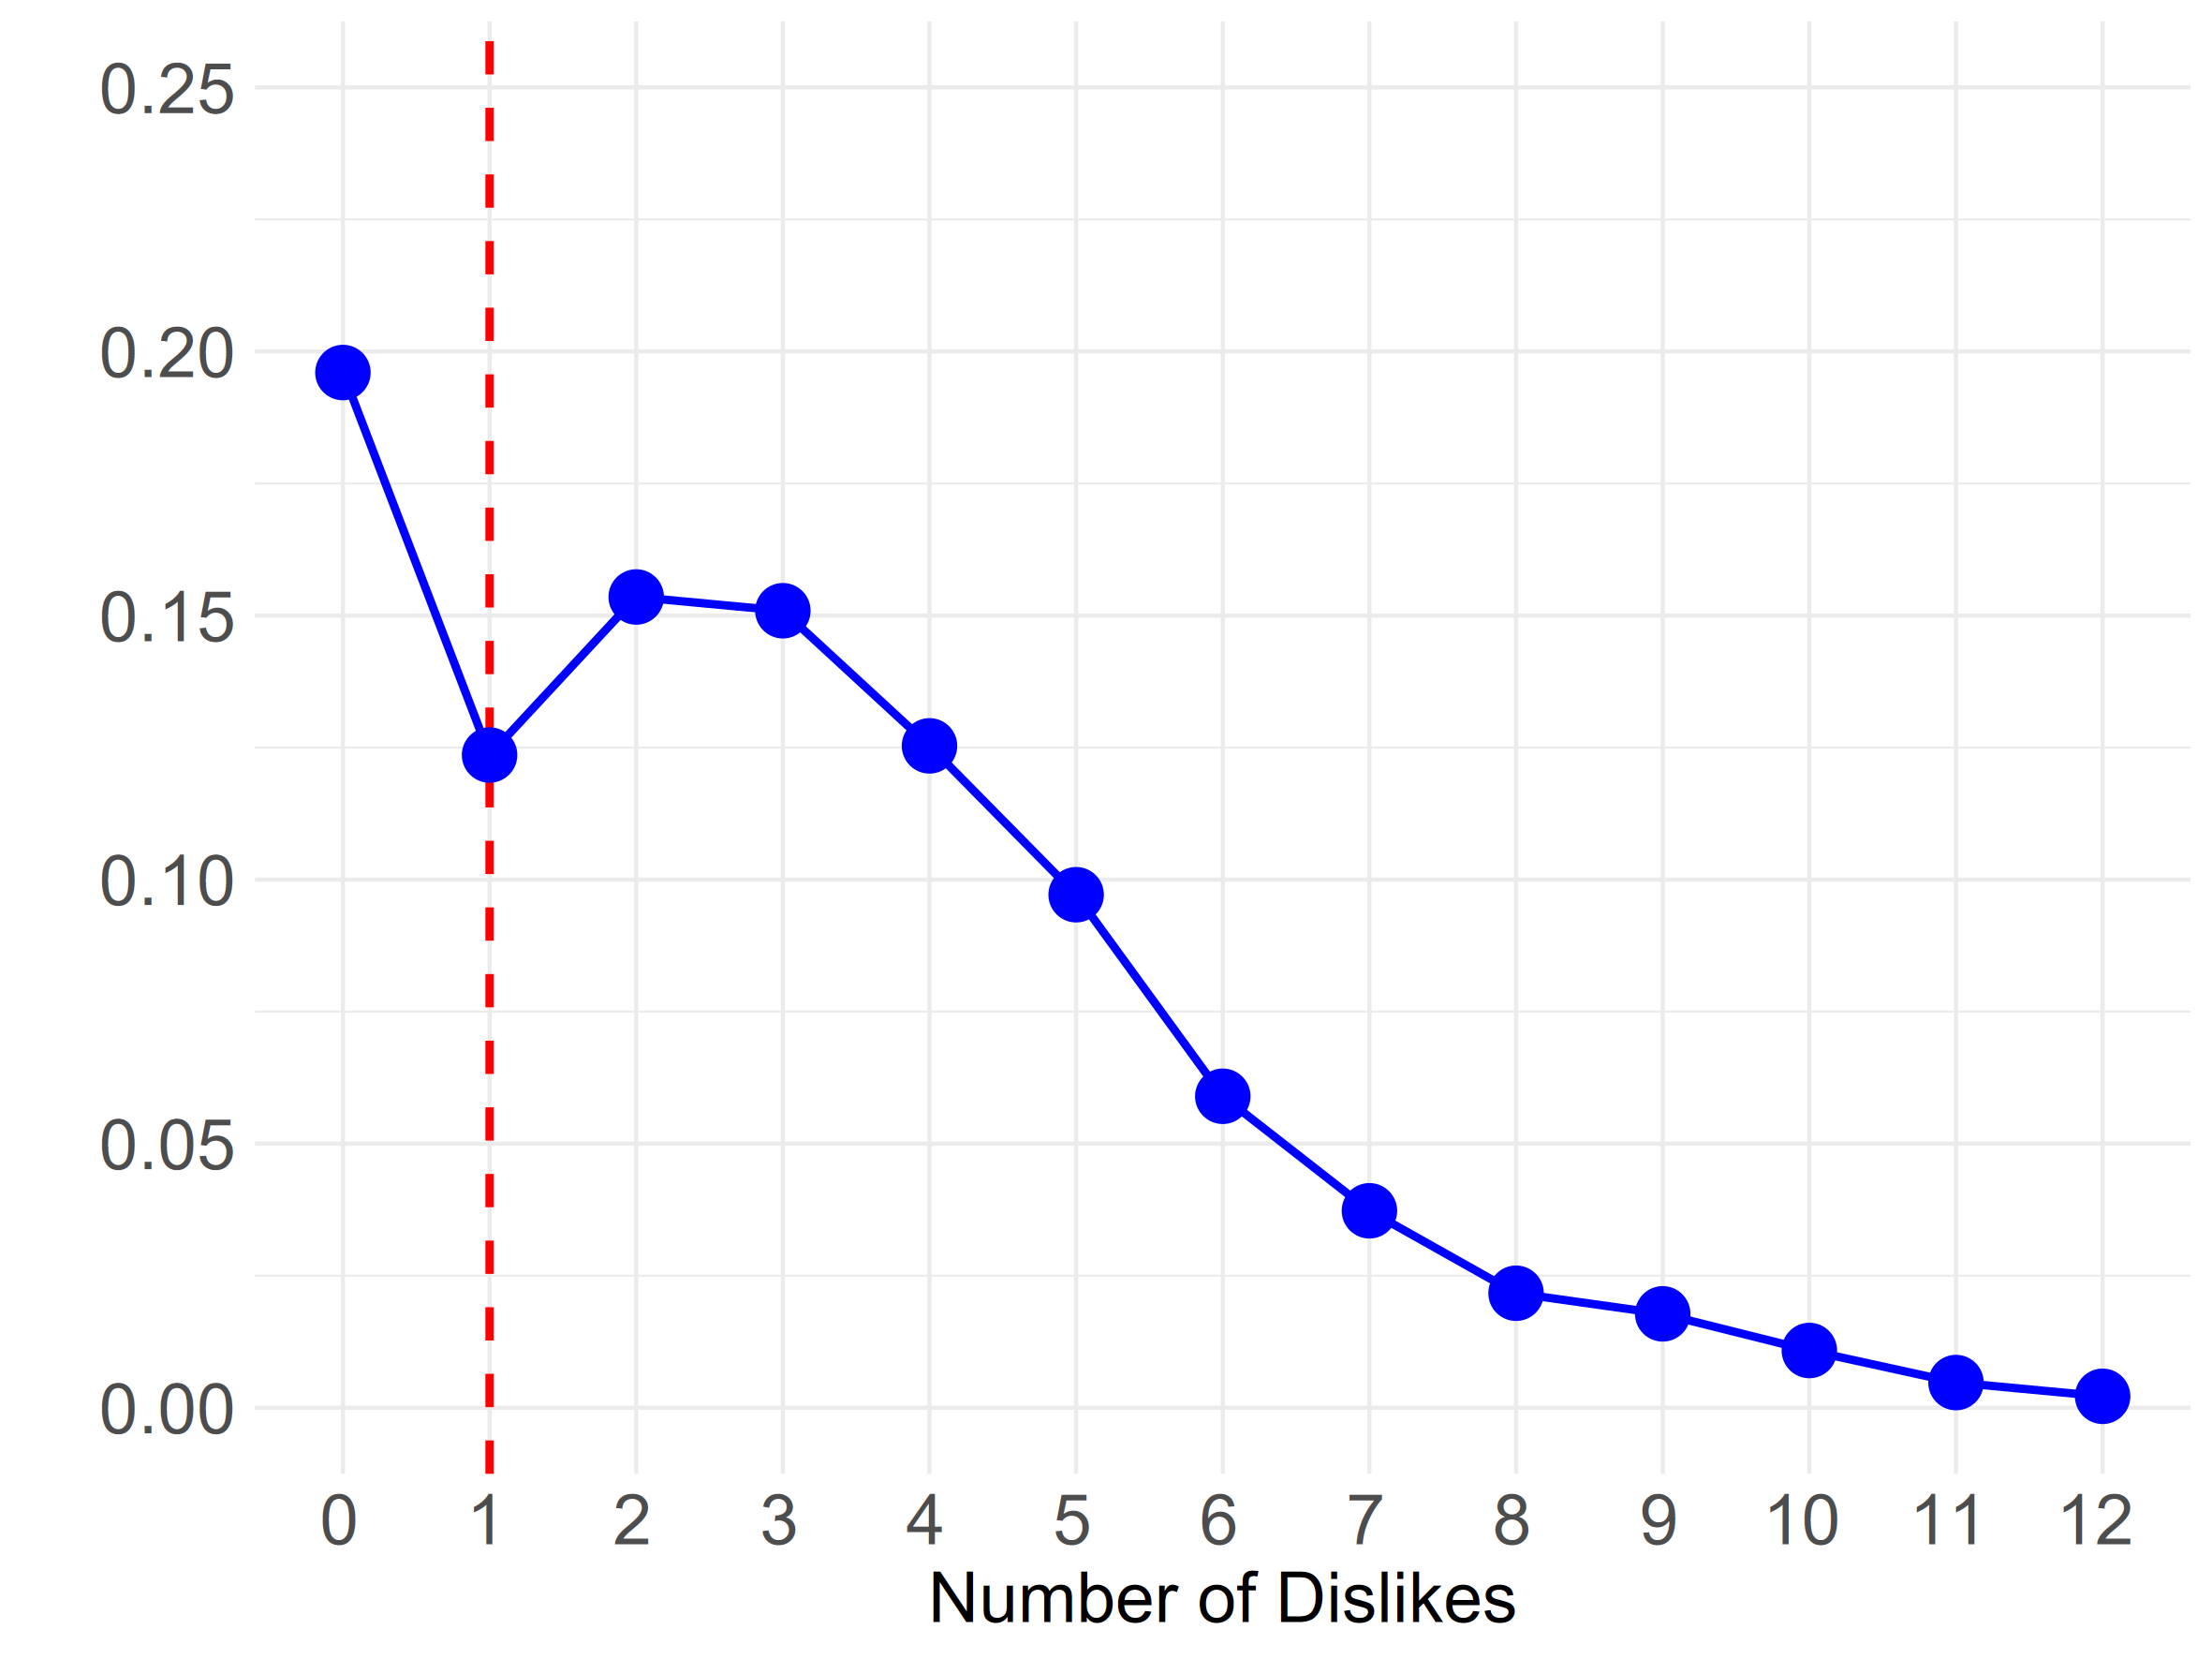
\includegraphics[width=1.0\textwidth]{Plots/uni-dist-cat-tol.png}
    \caption{Univariate plot of number of dislikes.}
    \label{fig:main}
\end{figure}
Figure~\ref{fig:main} shows the univariate distribution of the number of dislikes for the LM 2025 data. As we can see, the distribution exhibits excess zeroes, with about 20\% of the sample reporting zero dislikes among the twelve musical genres included. 


\begin{figure}[ht!]
    \captionsetup[subfigure]{font=footnotesize,labelfont=footnotesize}
    \centering
     \begin{subfigure}[b]{0.3\textwidth}
        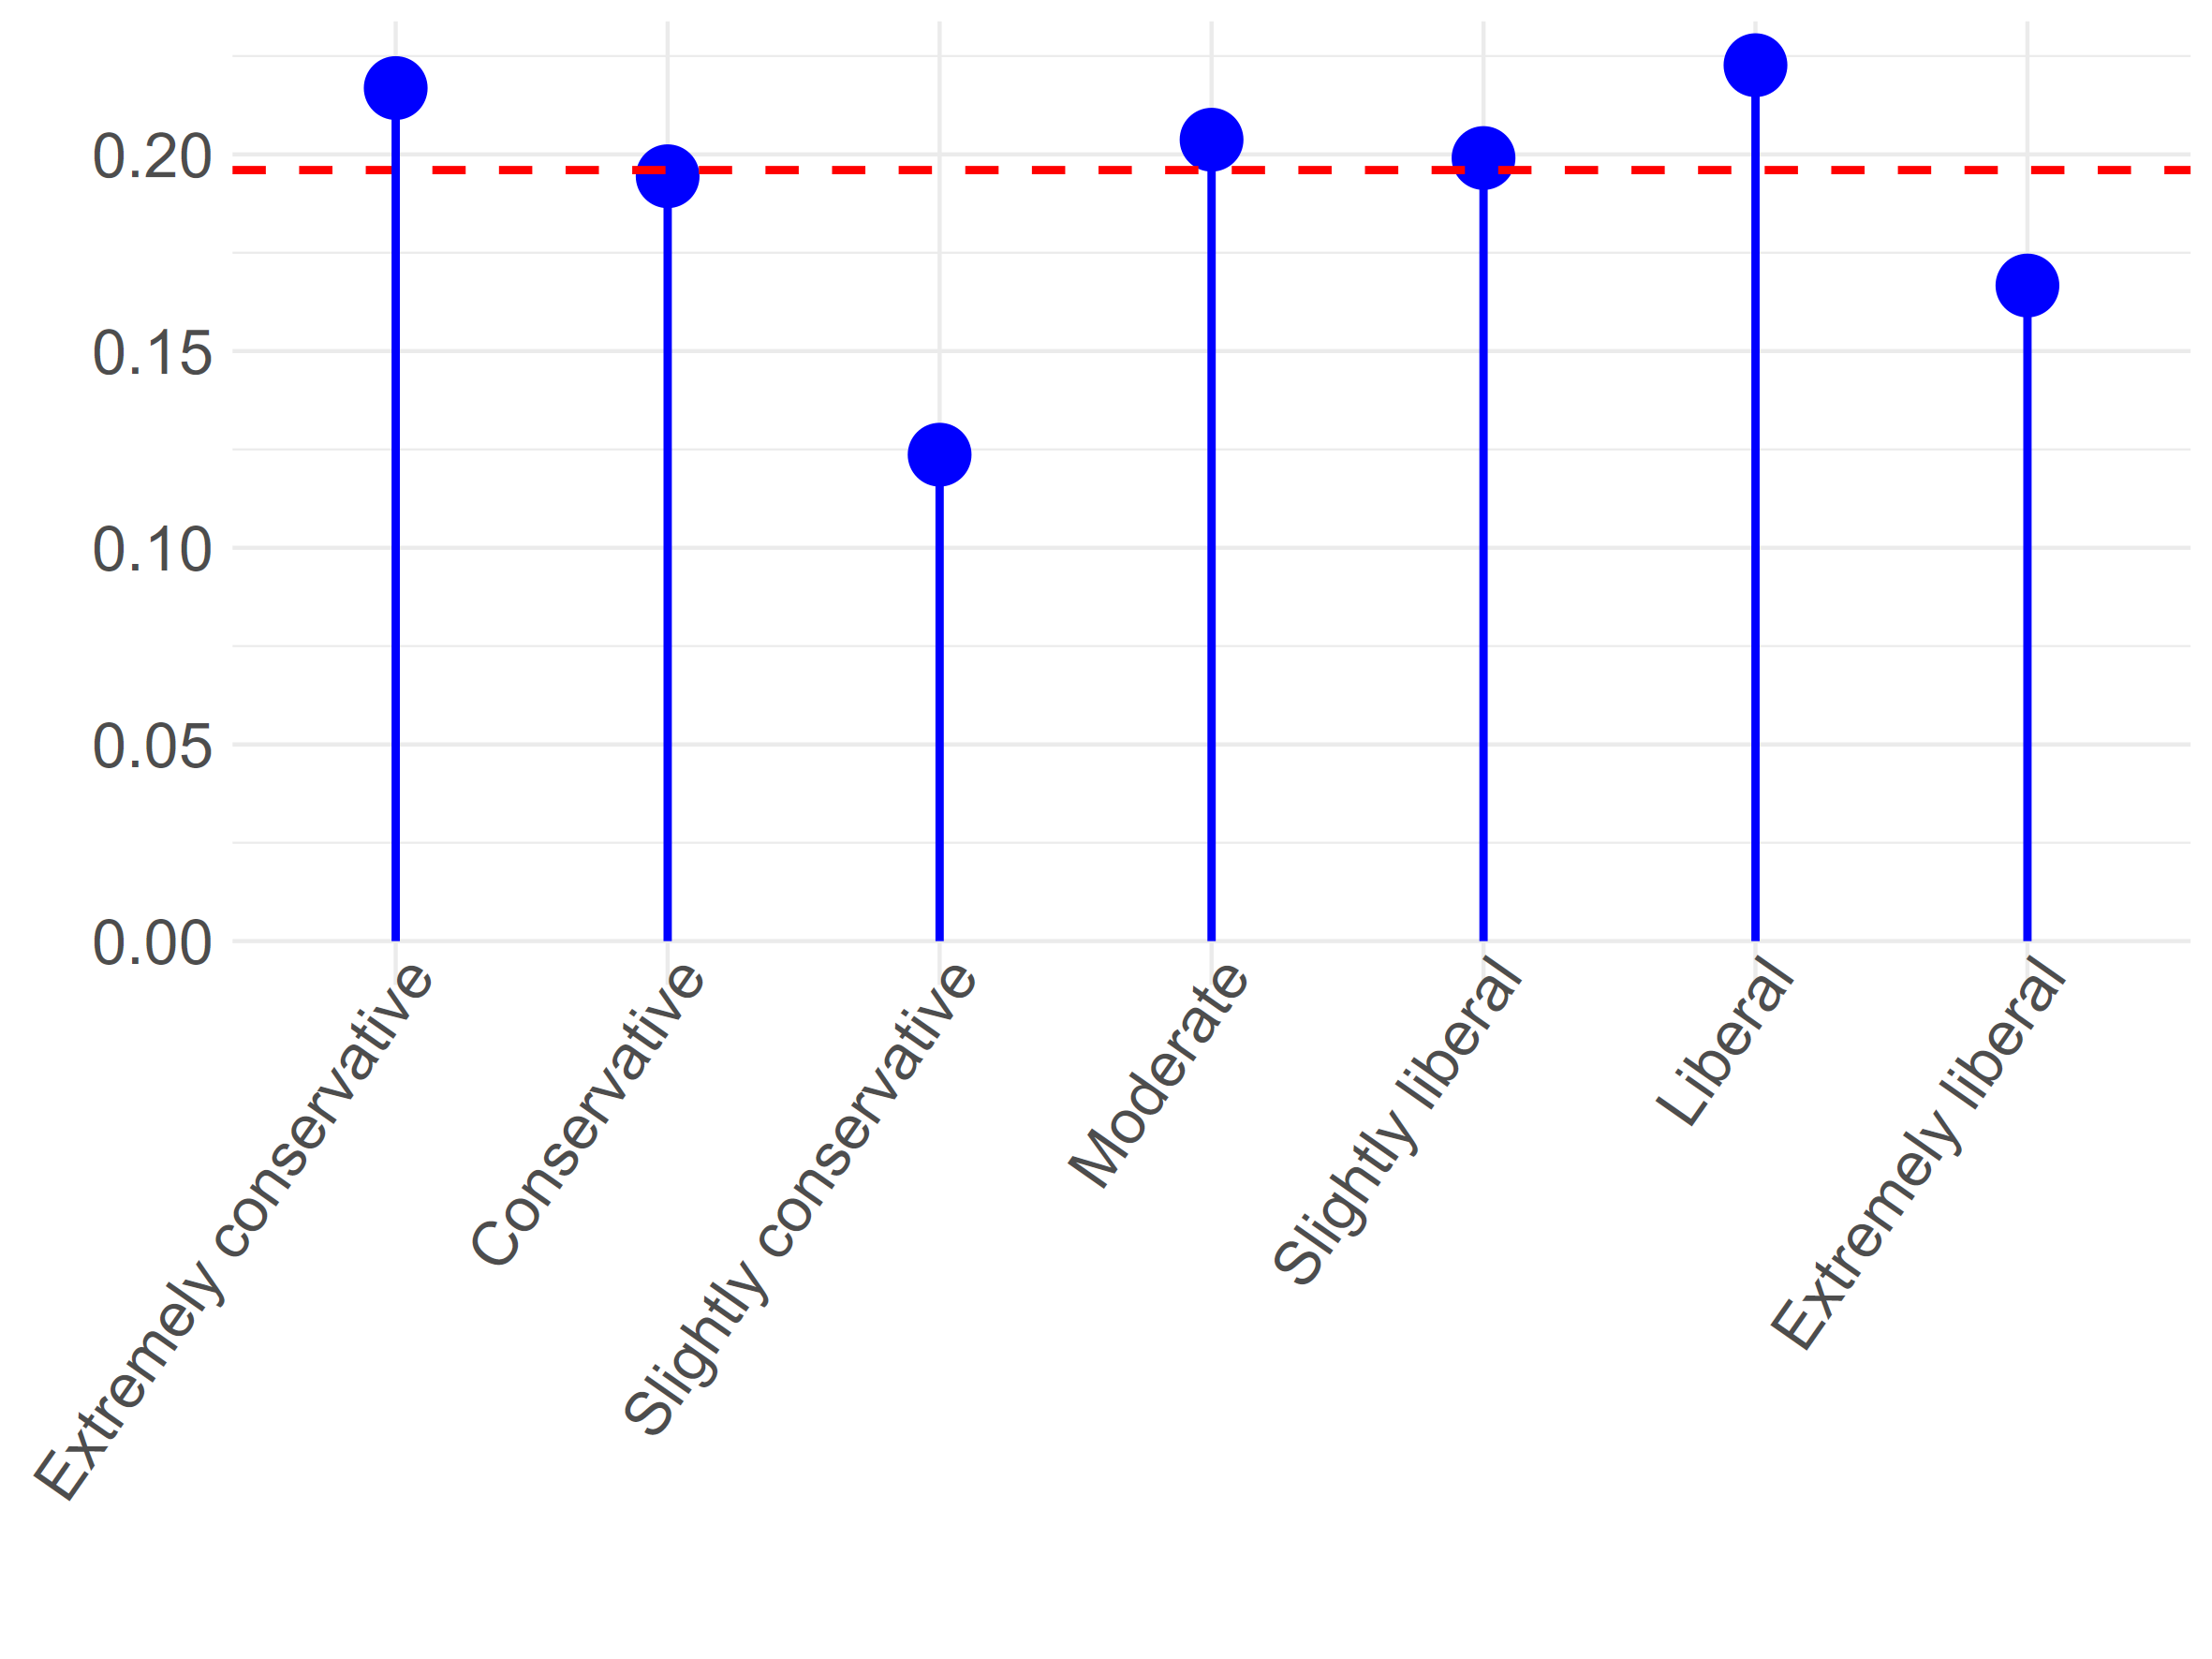
\includegraphics[width=1.0\textwidth]{Plots/uni-dist-cat-tol-pol.png}
            \caption{Political Ideology}
            \label{fig:cat-tol-pol}
    \end{subfigure}
     \begin{subfigure}[b]{0.3\textwidth}
        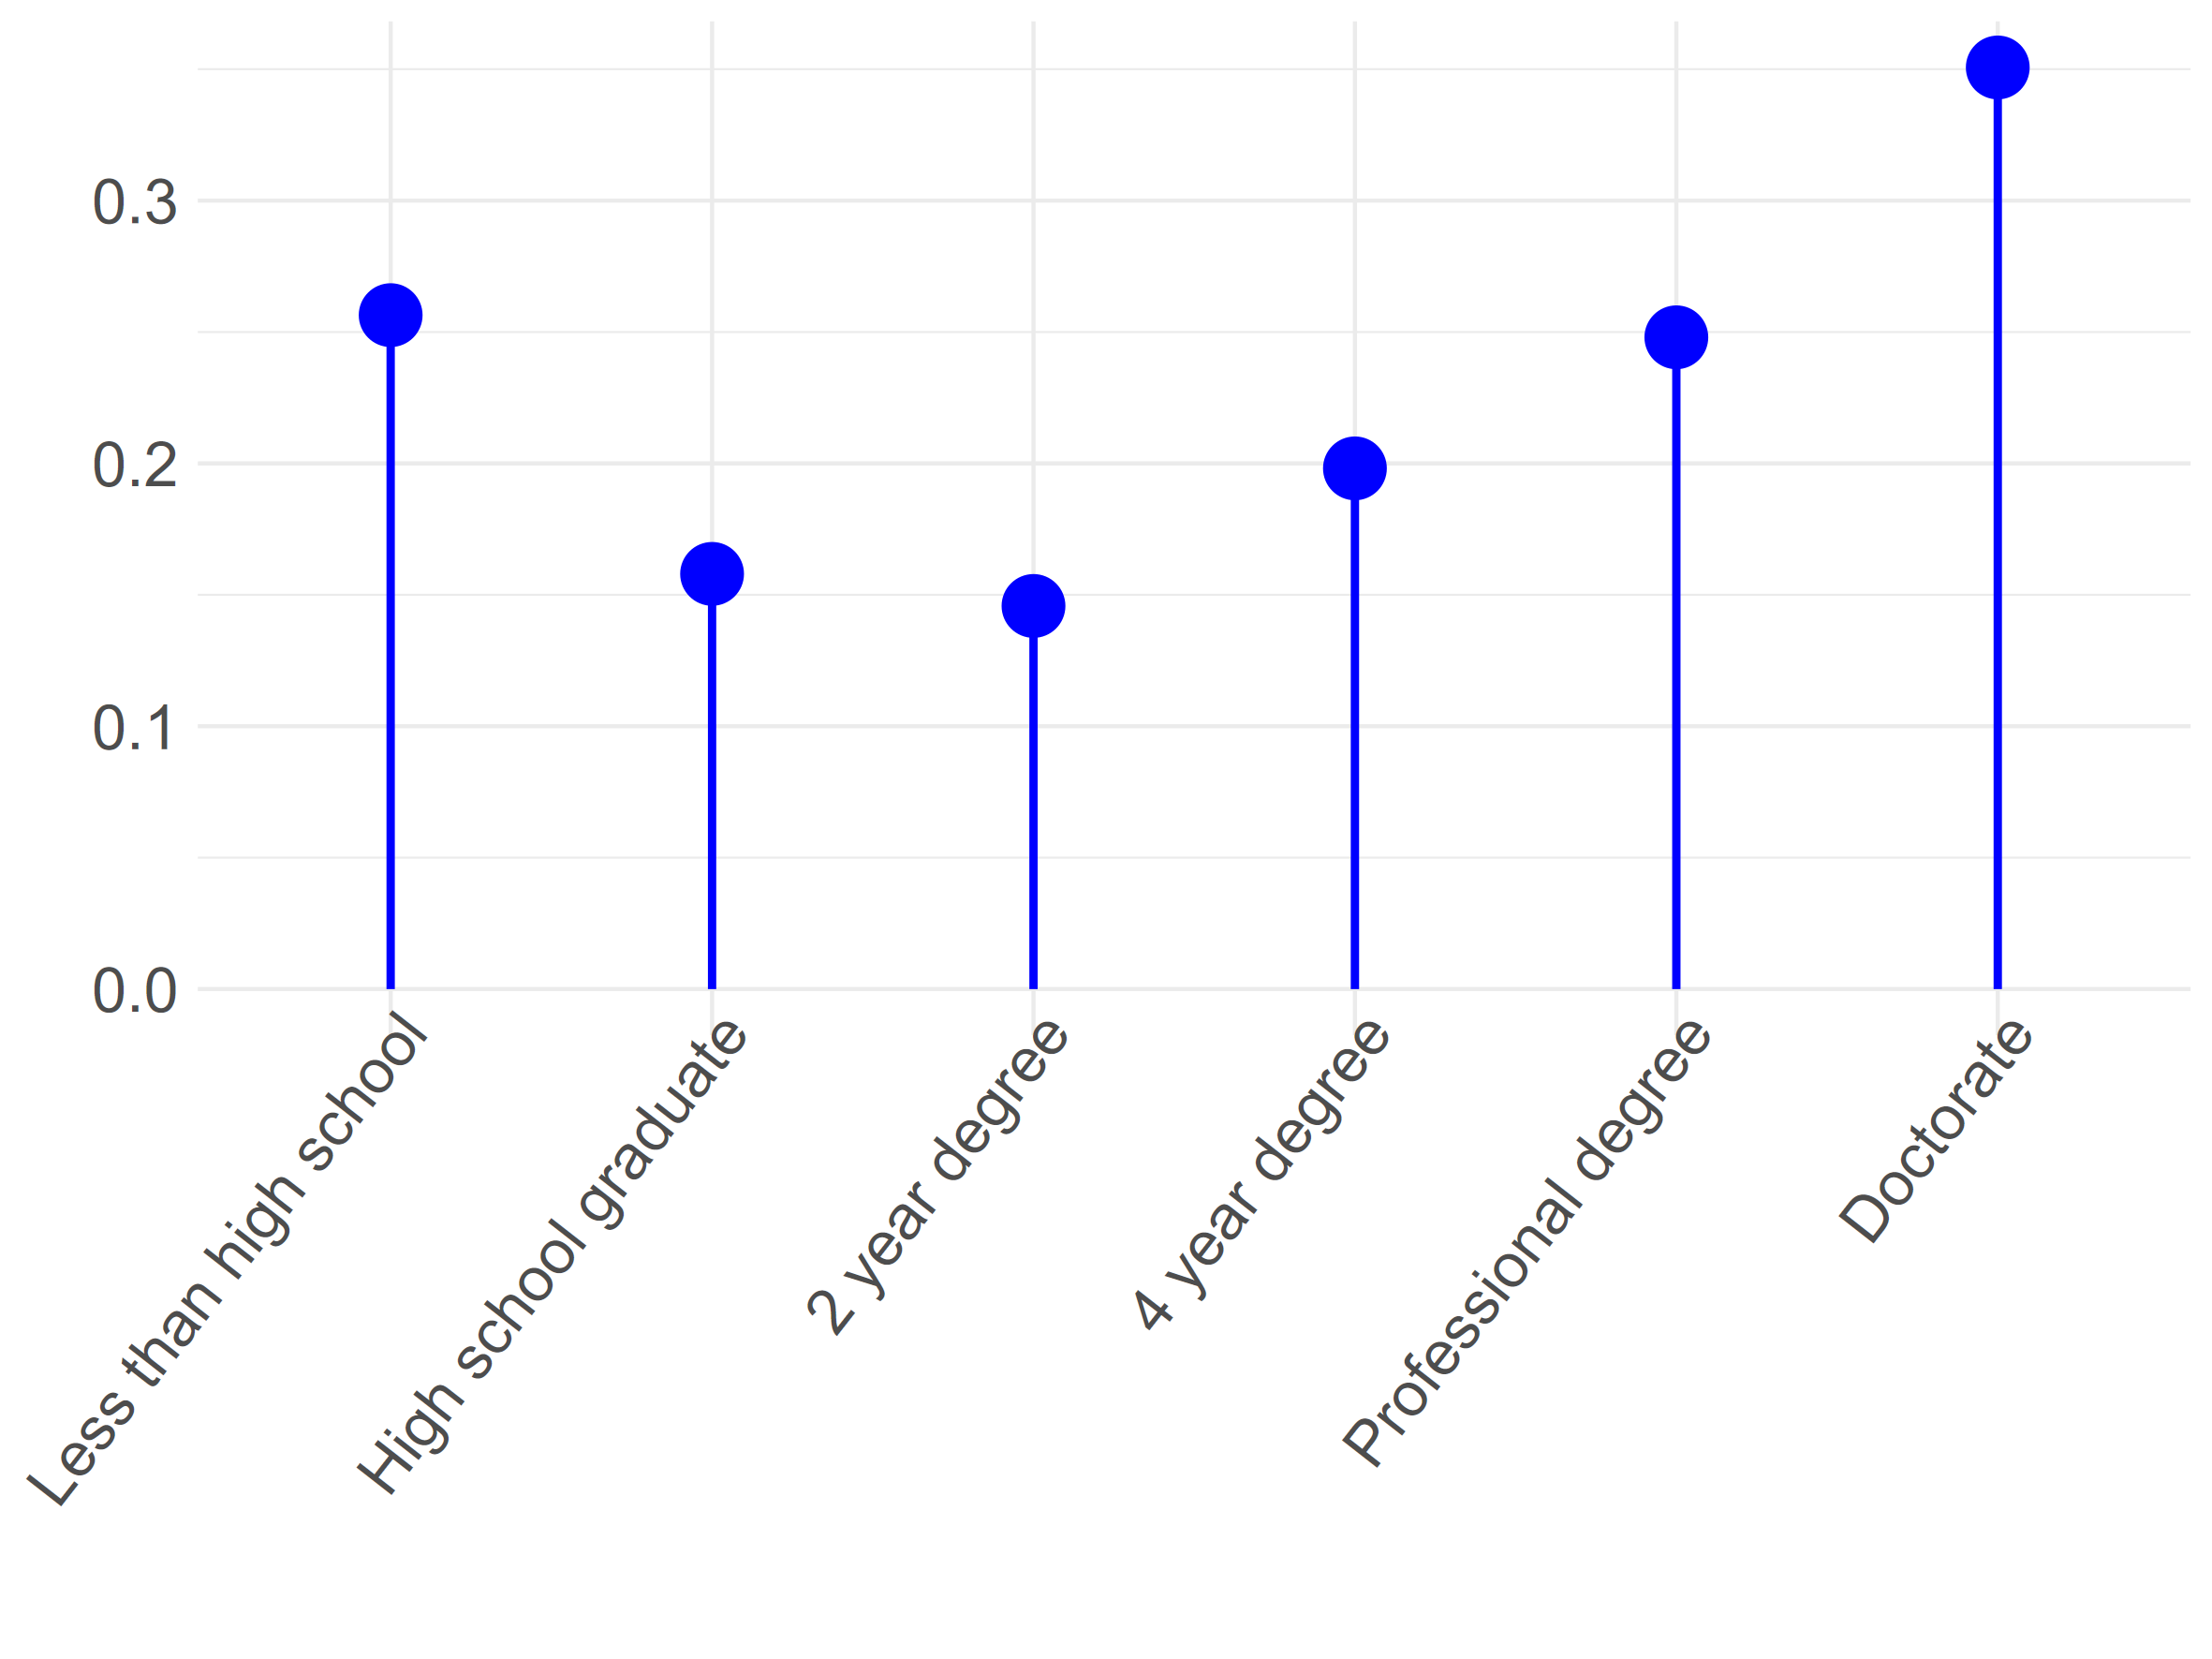
\includegraphics[width=1.0\textwidth]{Plots/uni-dist-cat-tol-edu.png}
            \caption{Education}
            \label{fig:cat-tol-edu}
    \end{subfigure}
     \begin{subfigure}[b]{0.3\textwidth}
        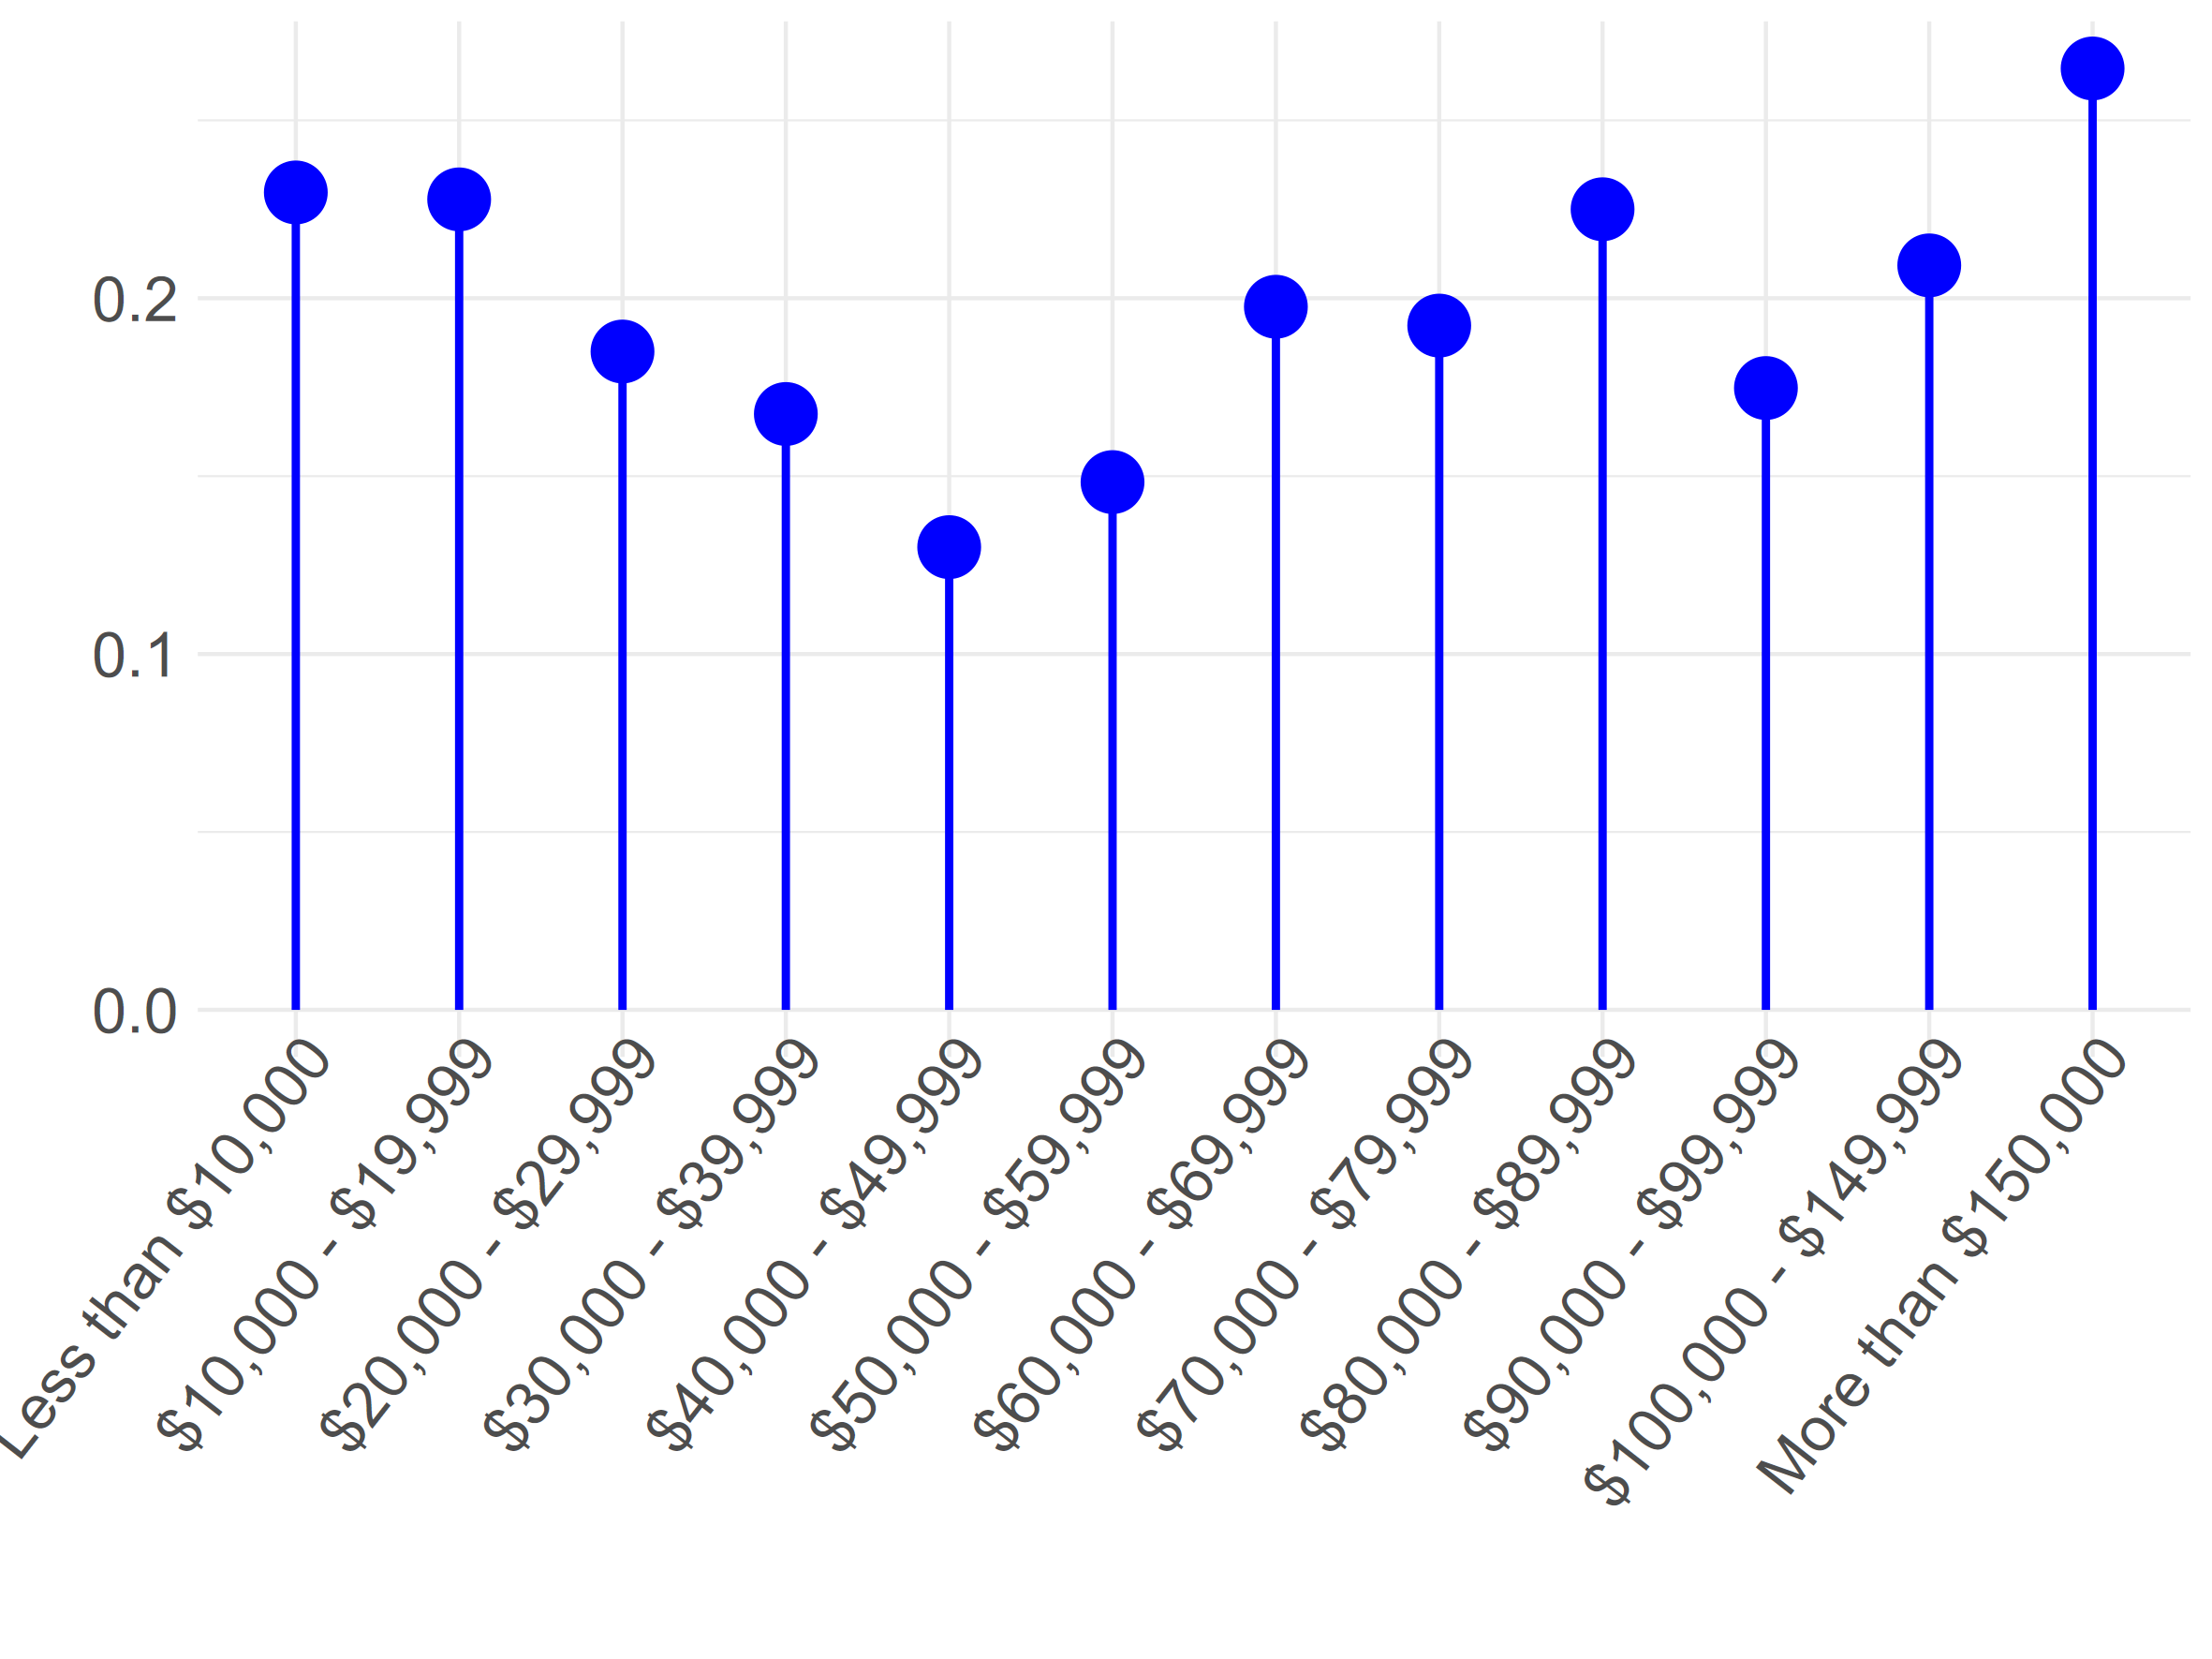
\includegraphics[width=1.0\textwidth]{Plots/uni-dist-cat-tol-inc.png}
            \caption{Income}
            \label{fig:cat-tol-inc}
    \end{subfigure}
     \begin{subfigure}[b]{0.3\textwidth}
        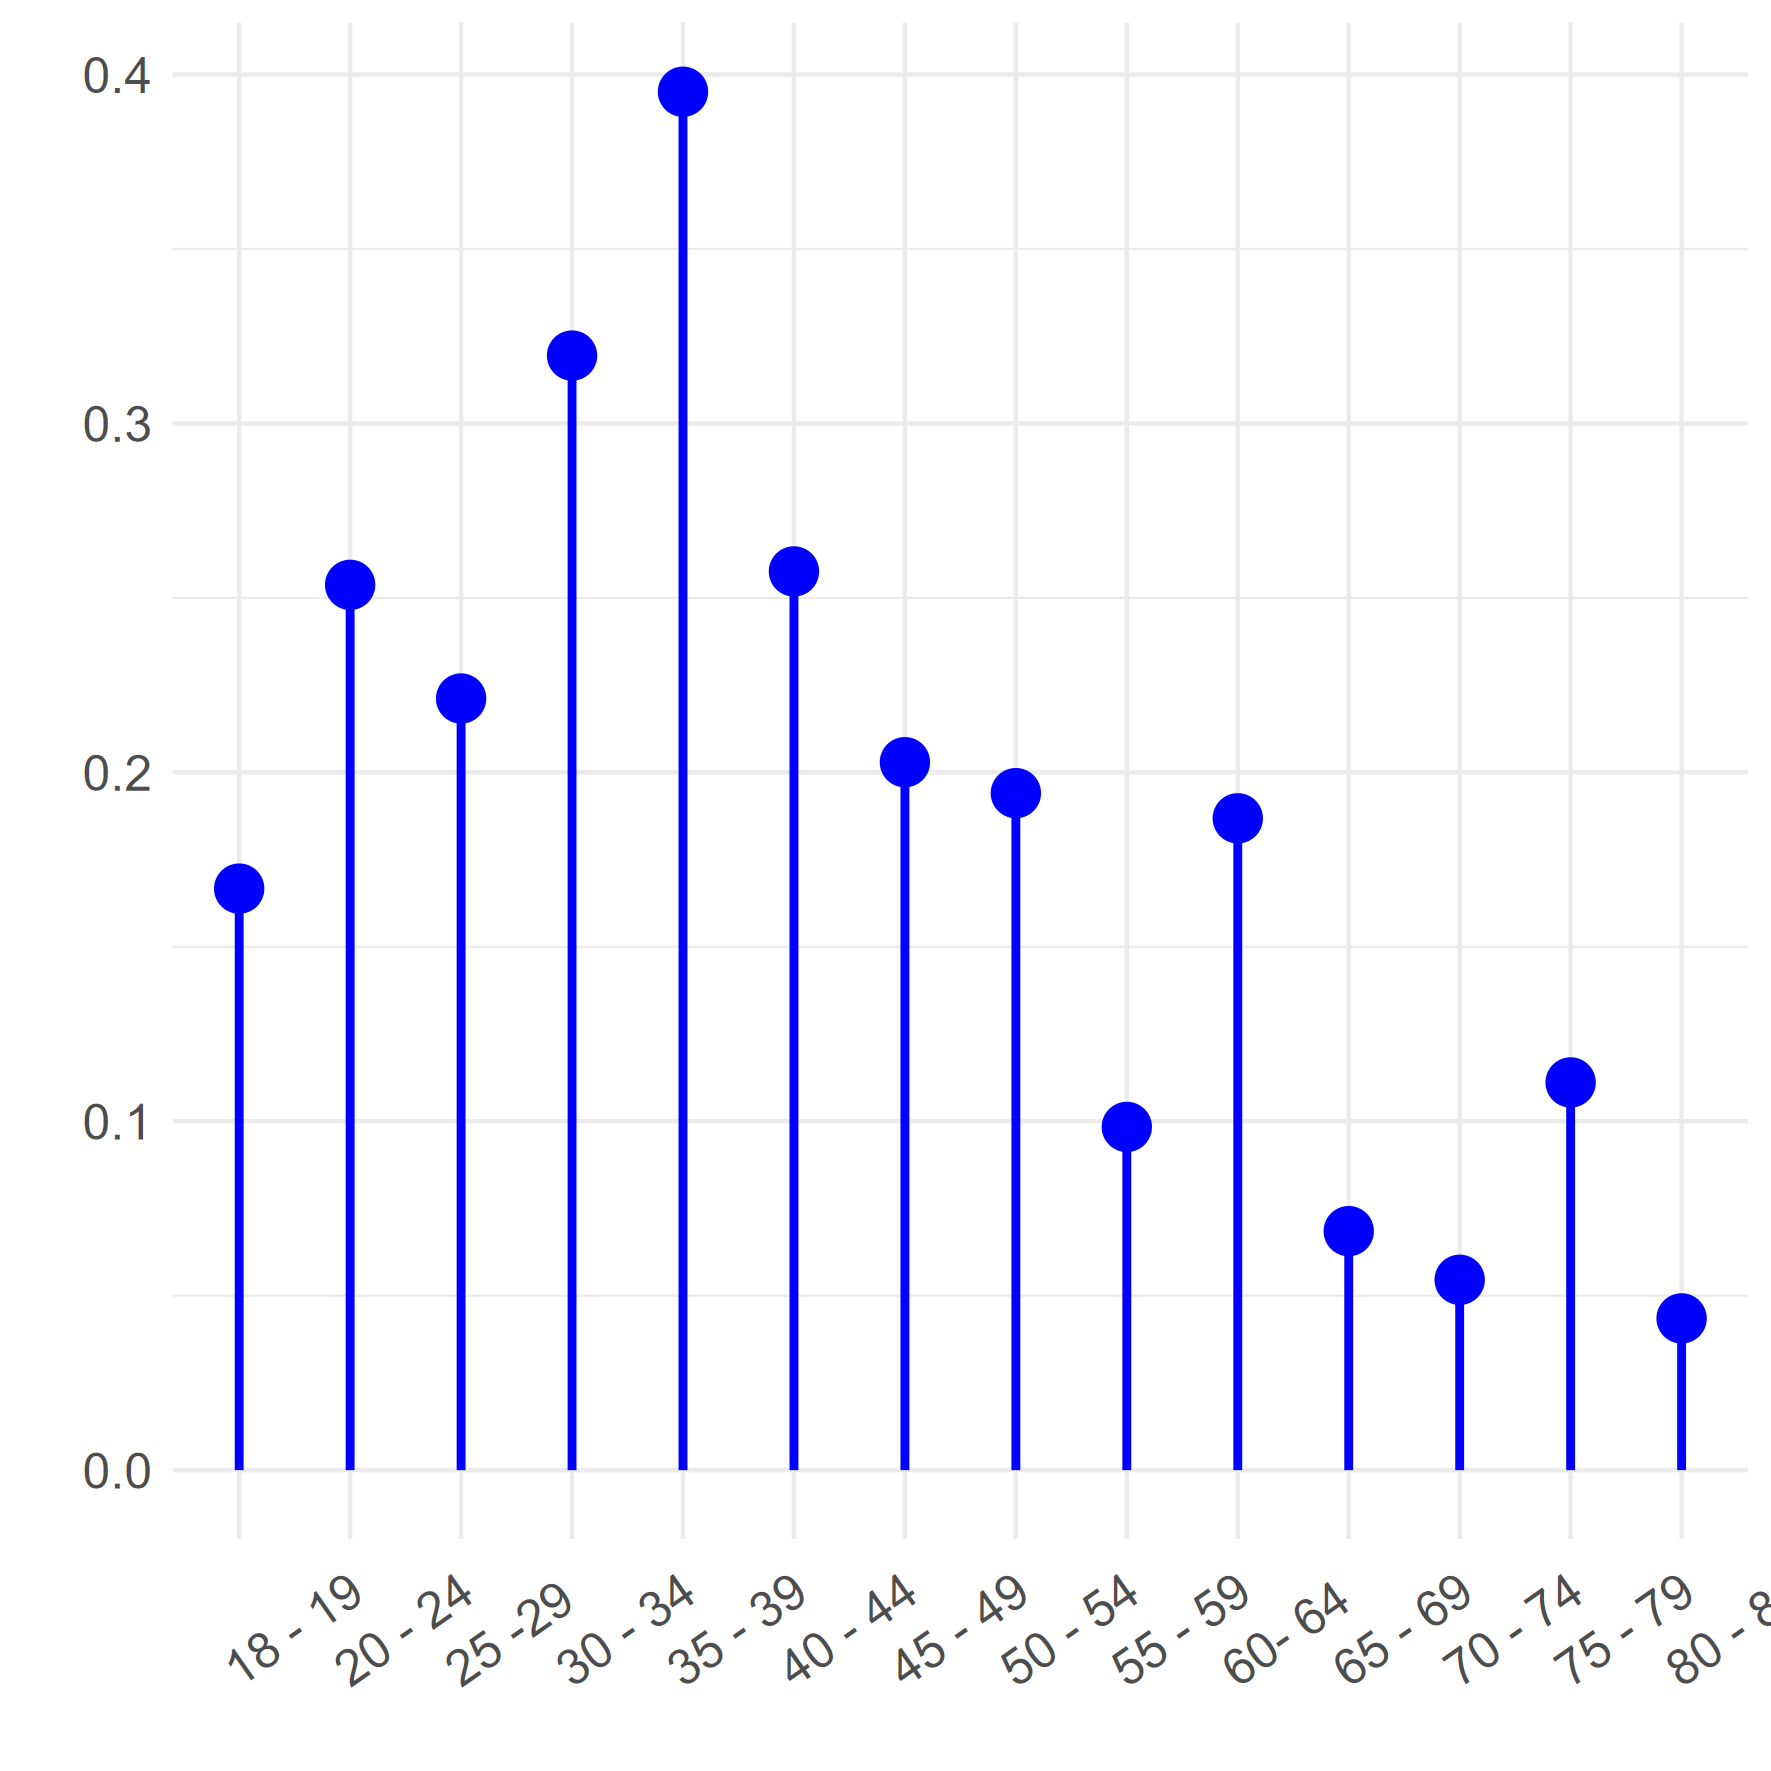
\includegraphics[width=1.0\textwidth]{Plots/uni-dist-cat-tol-age.png}
            \caption{Age}
            \label{fig:cat-tol-age}
    \end{subfigure}
     \begin{subfigure}[b]{0.3\textwidth}
        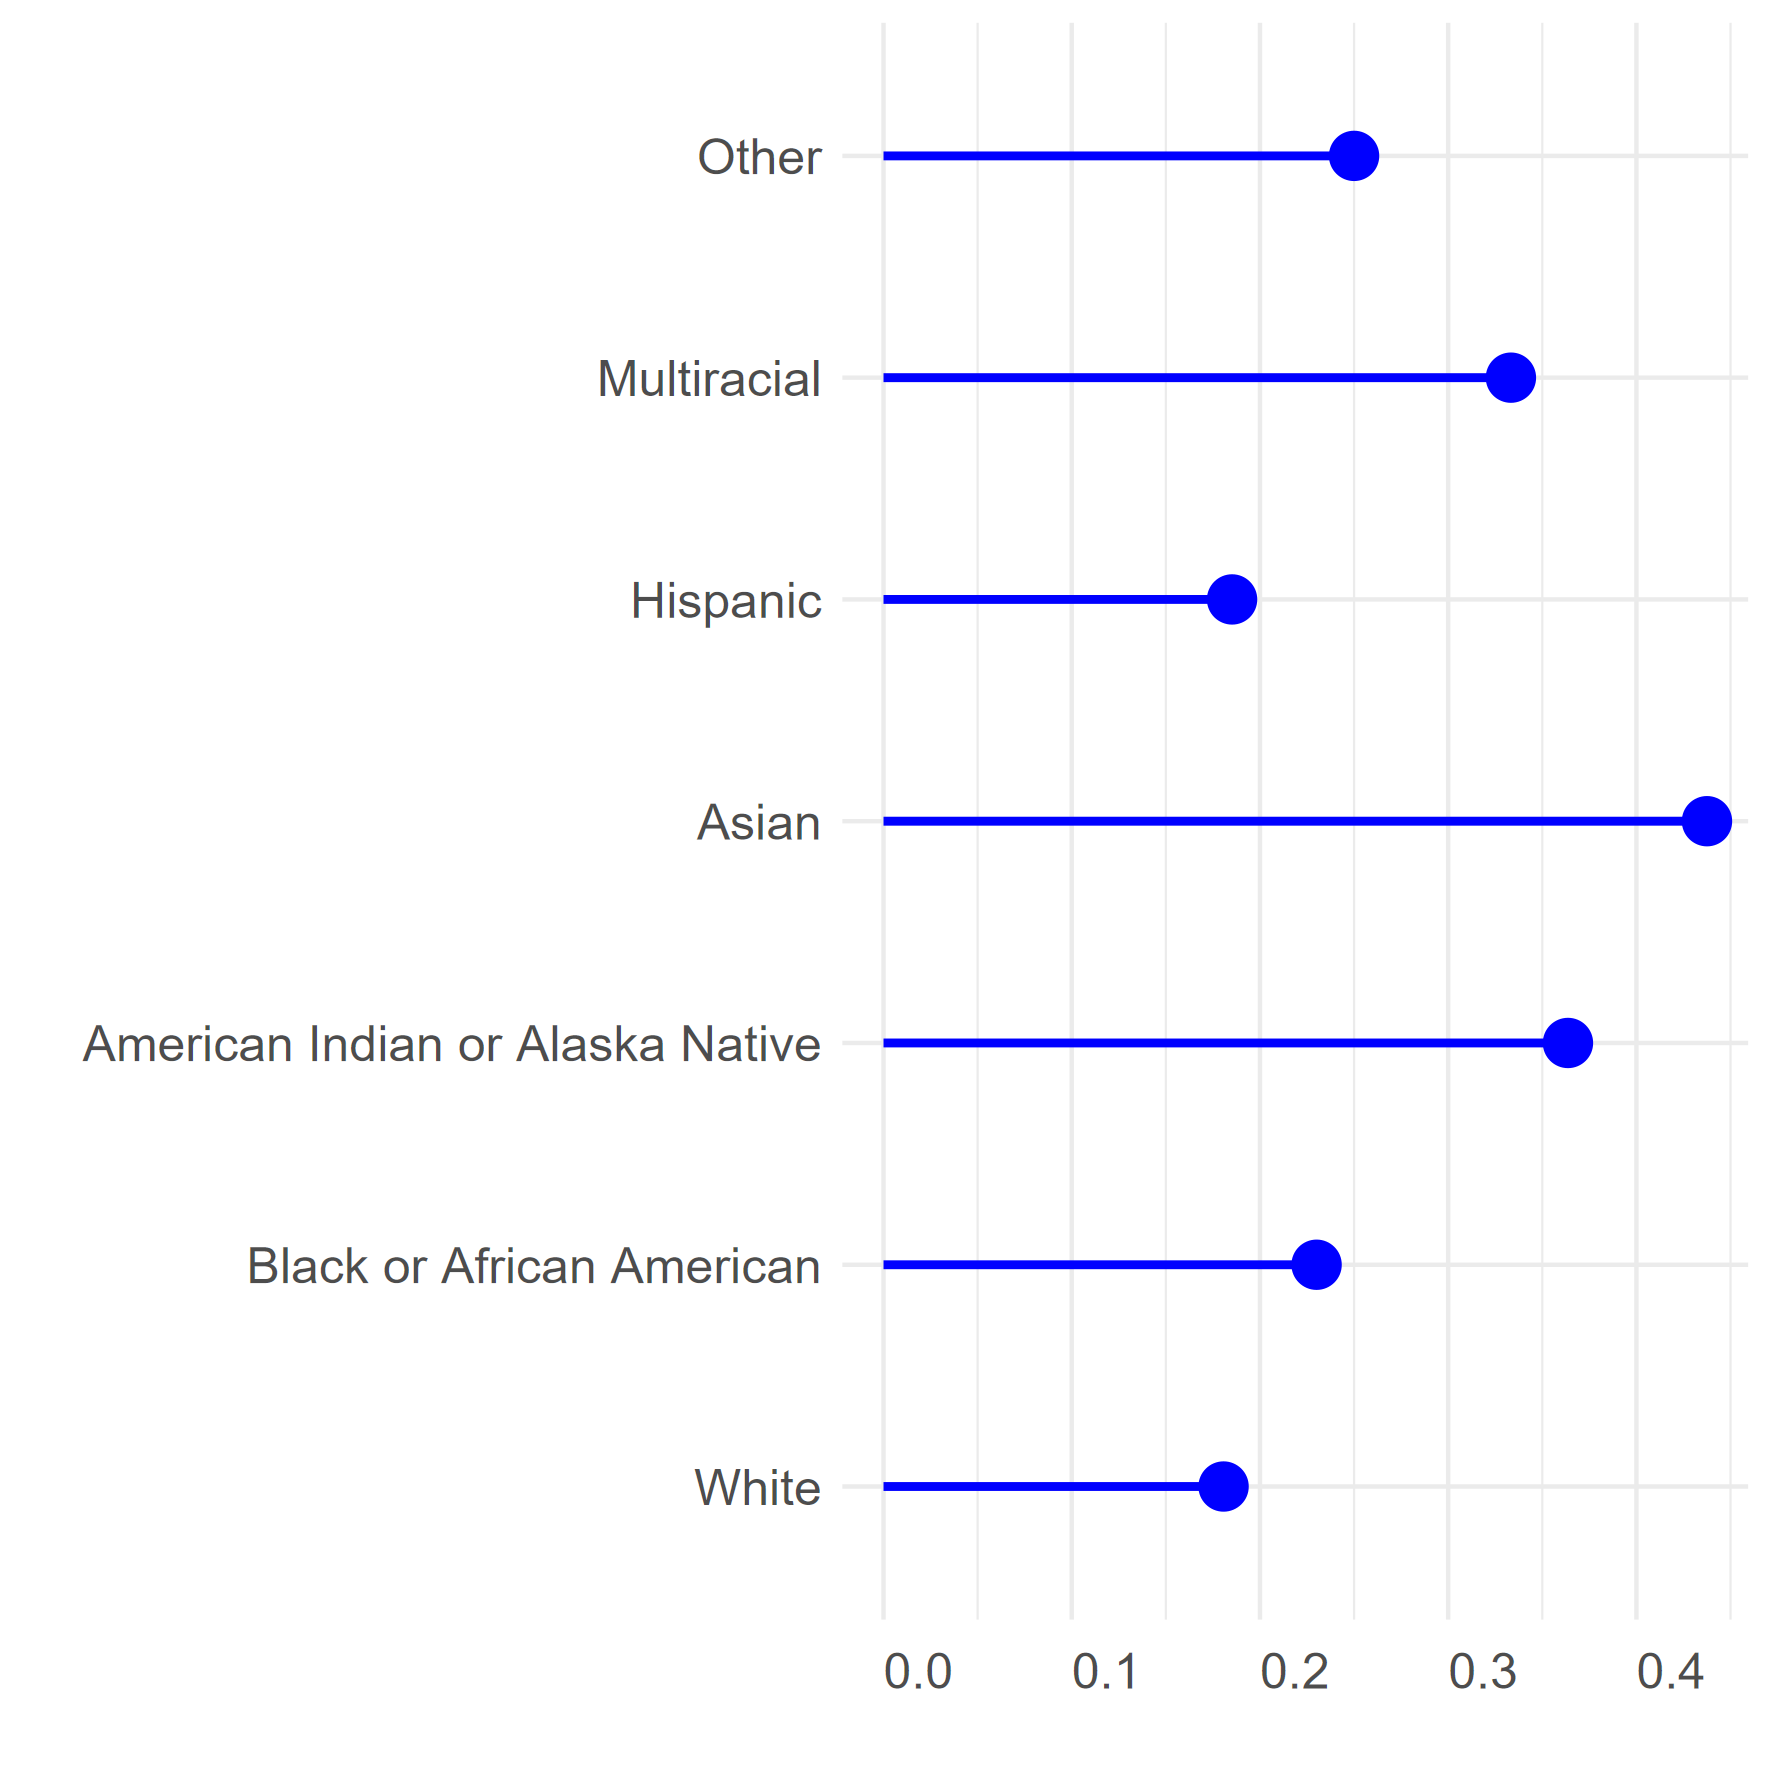
\includegraphics[width=1.0\textwidth]{Plots/uni-dist-cat-tol-rac.png}
            \caption{Ethnoracial Identification}
            \label{fig:cat-tol-rac}
    \end{subfigure}
     \begin{subfigure}[b]{0.3\textwidth}
        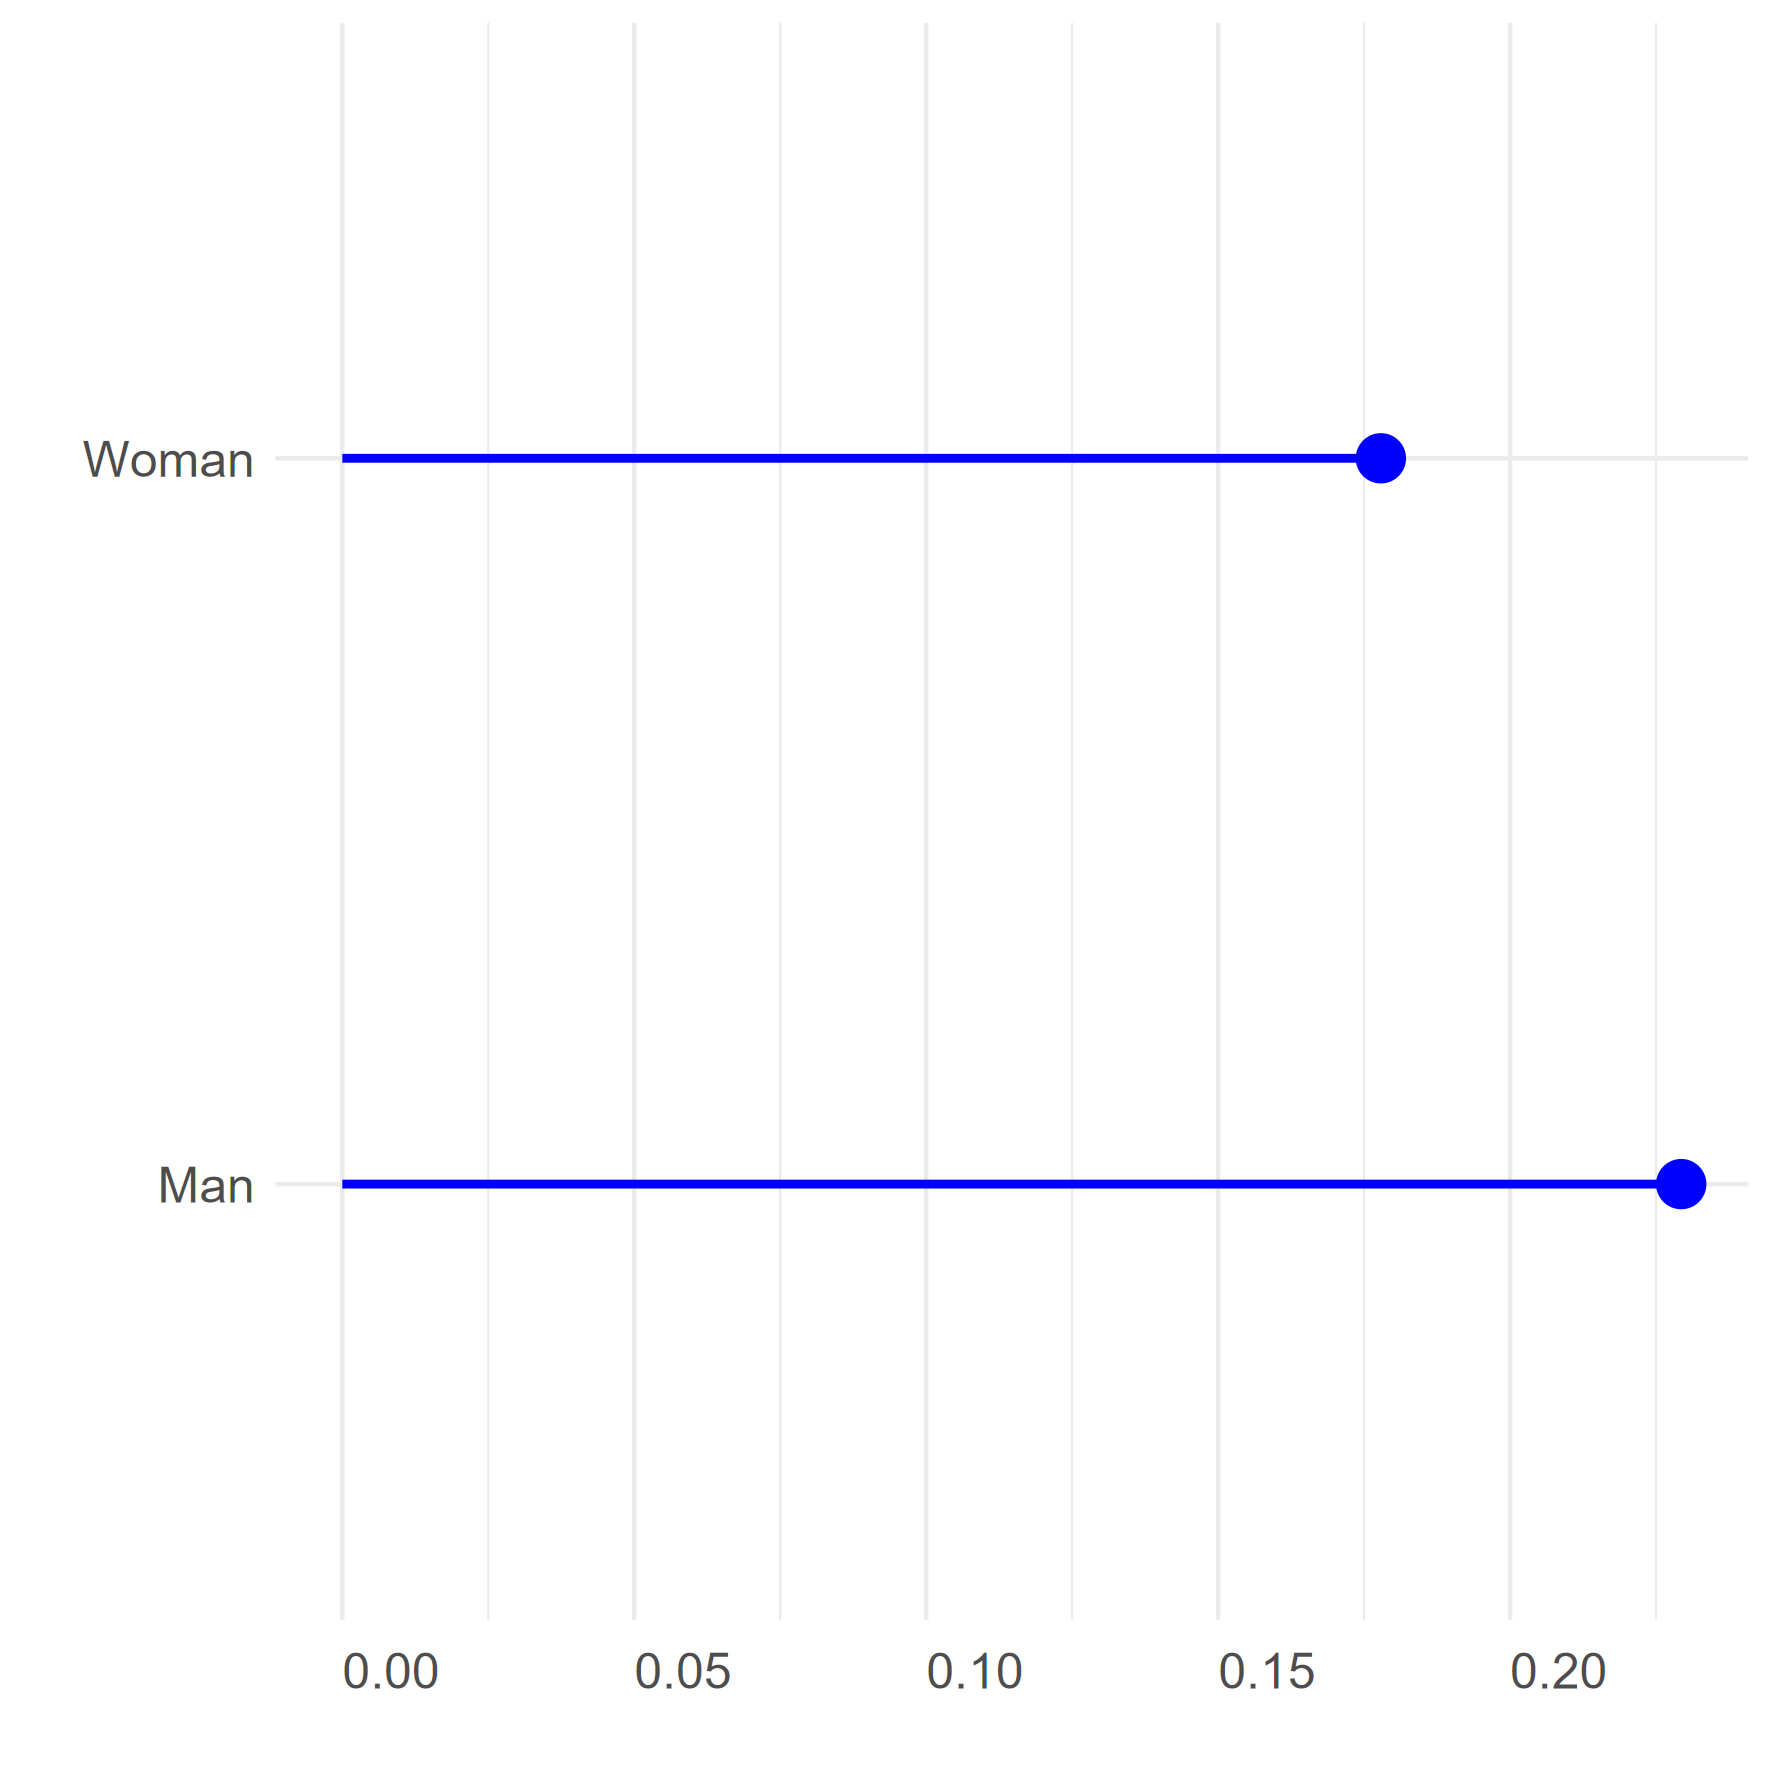
\includegraphics[width=1.0\textwidth]{Plots/uni-dist-cat-tol-gen.png}
            \caption{Gender Identification}
            \label{fig:cat-tol-gen}
    \end{subfigure}
    \caption{Proportion of Categorical Tolerants across different socio-demographic characteristics.}
    \label{fig:cat-tol}
\end{figure}

\begin{figure}[ht!]
    \captionsetup[subfigure]{font=footnotesize,labelfont=footnotesize}
    \centering
     \begin{subfigure}[b]{0.3\textwidth}
        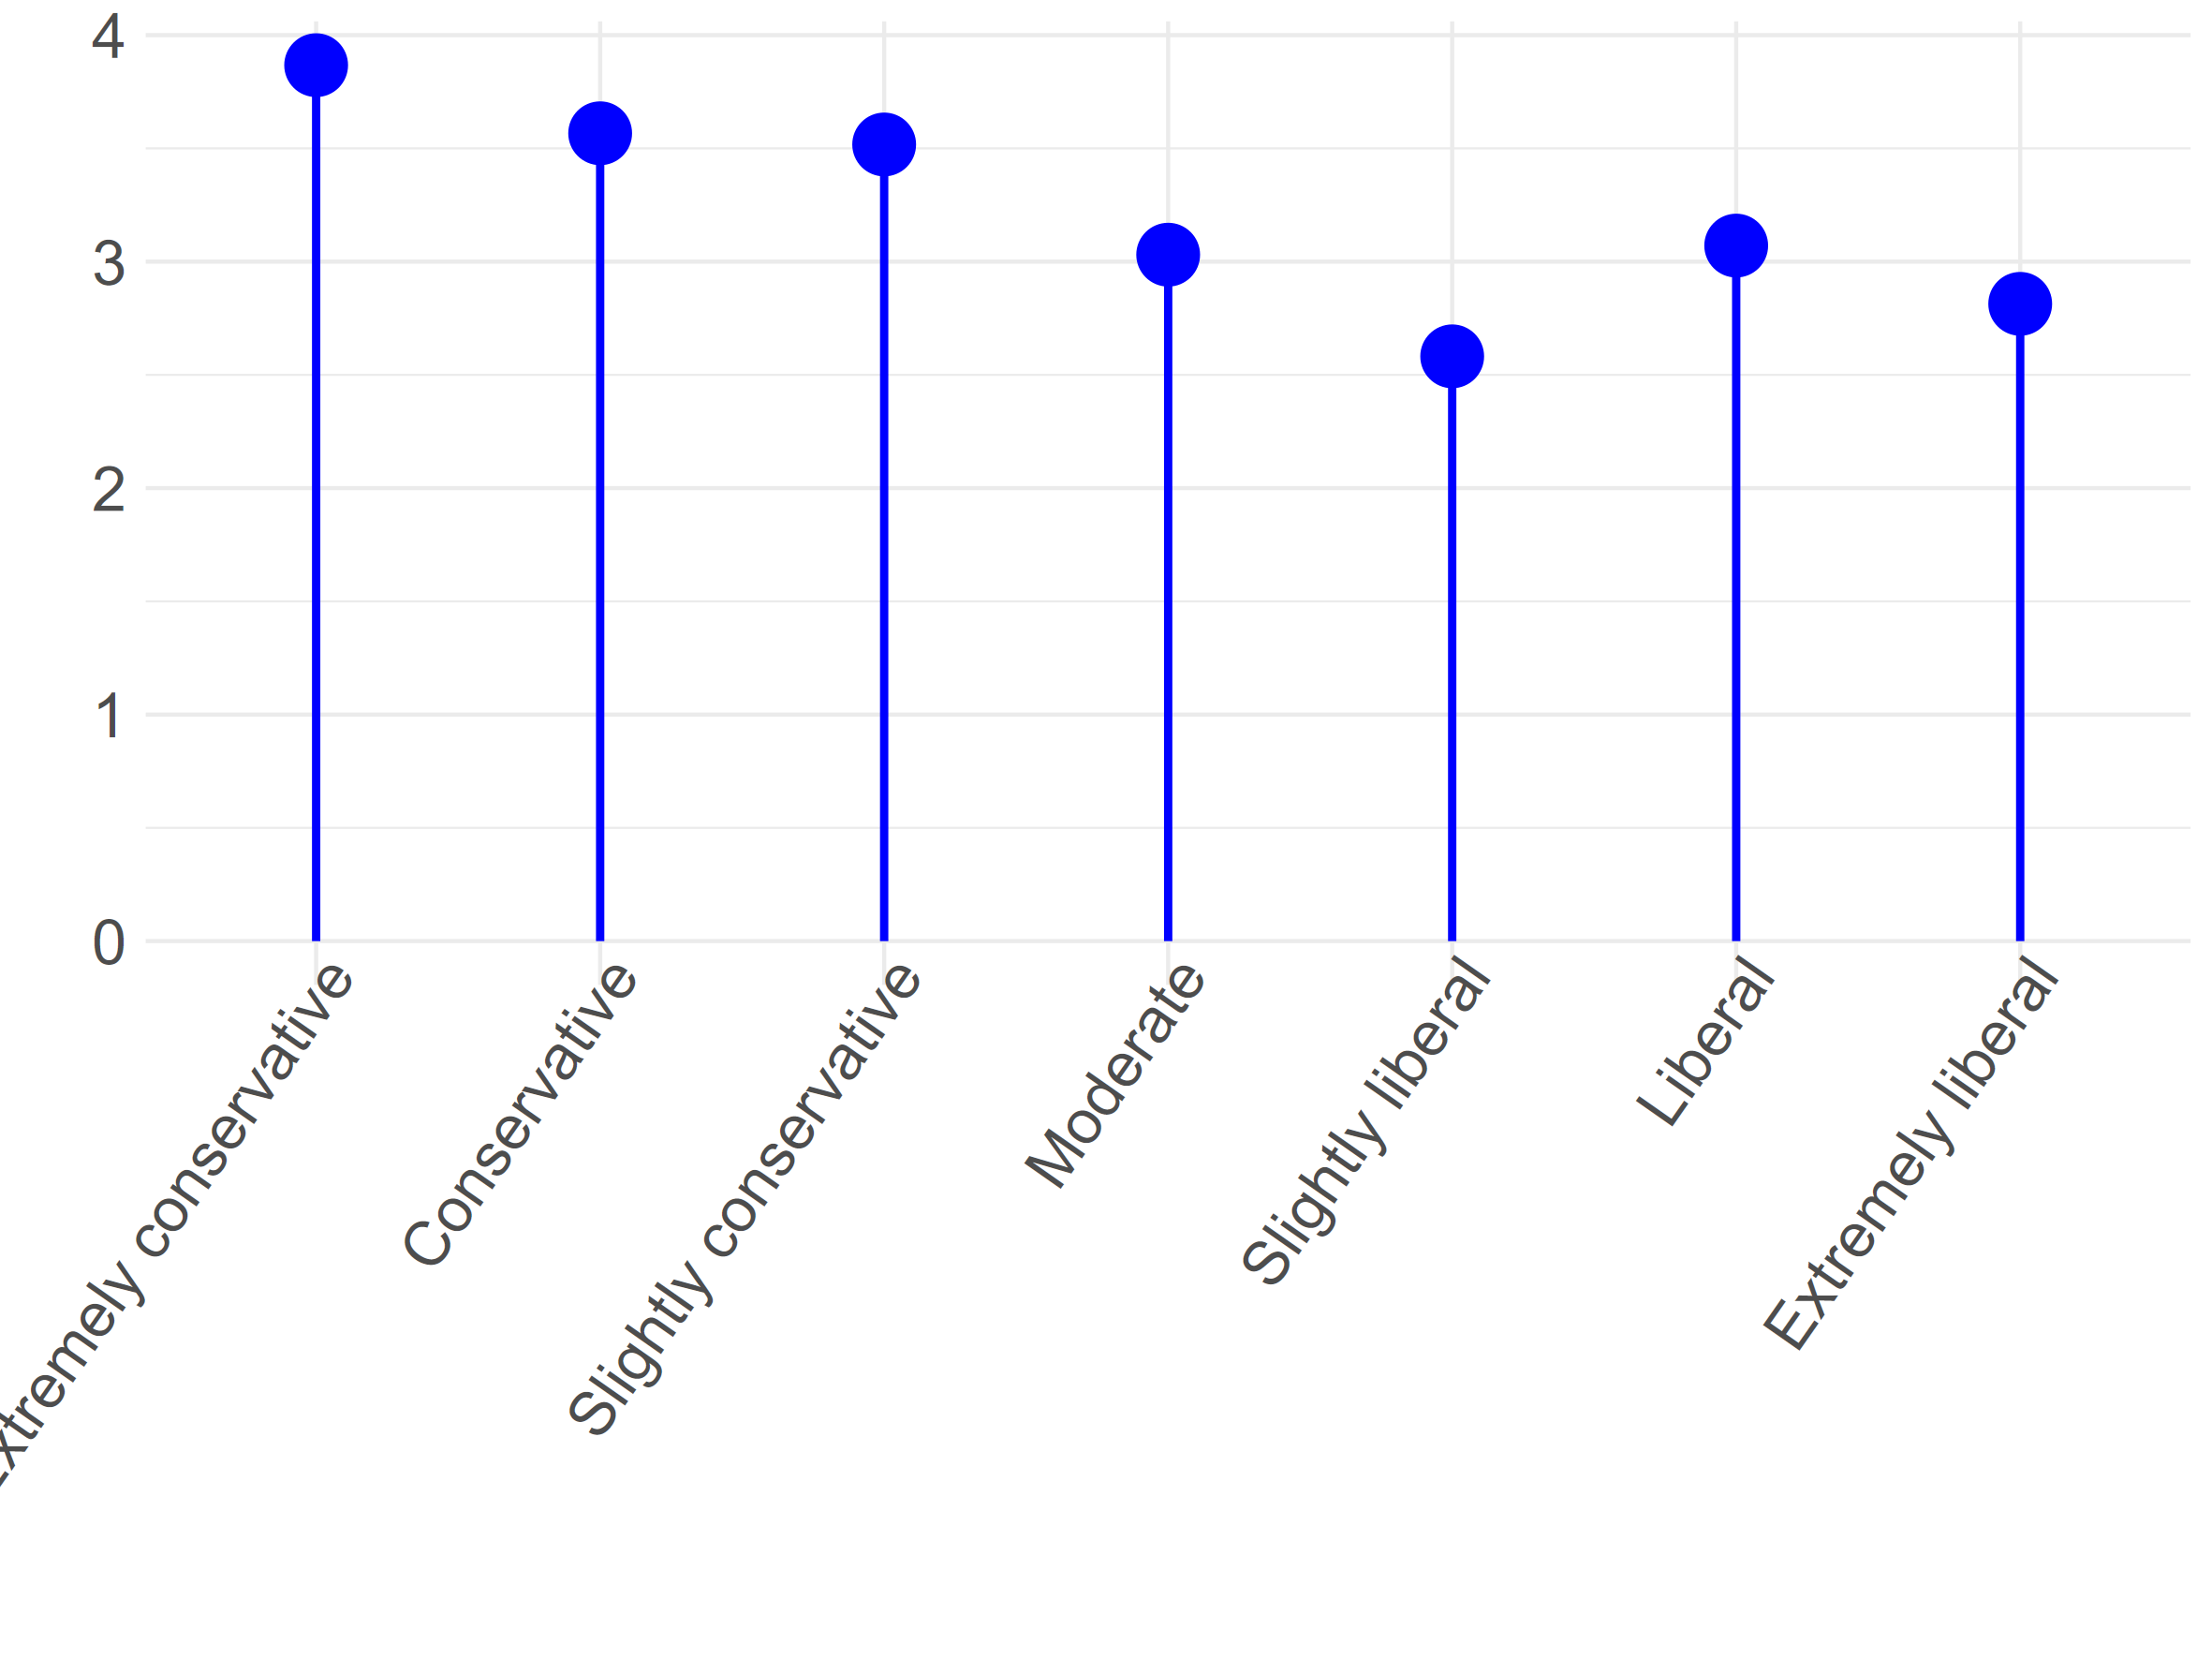
\includegraphics[width=1.0\textwidth]{Plots/uni-dist-grd-int-pol.png}
            \caption{Political Ideology}
            \label{fig:grd-int-pol}
    \end{subfigure}
     \begin{subfigure}[b]{0.3\textwidth}
        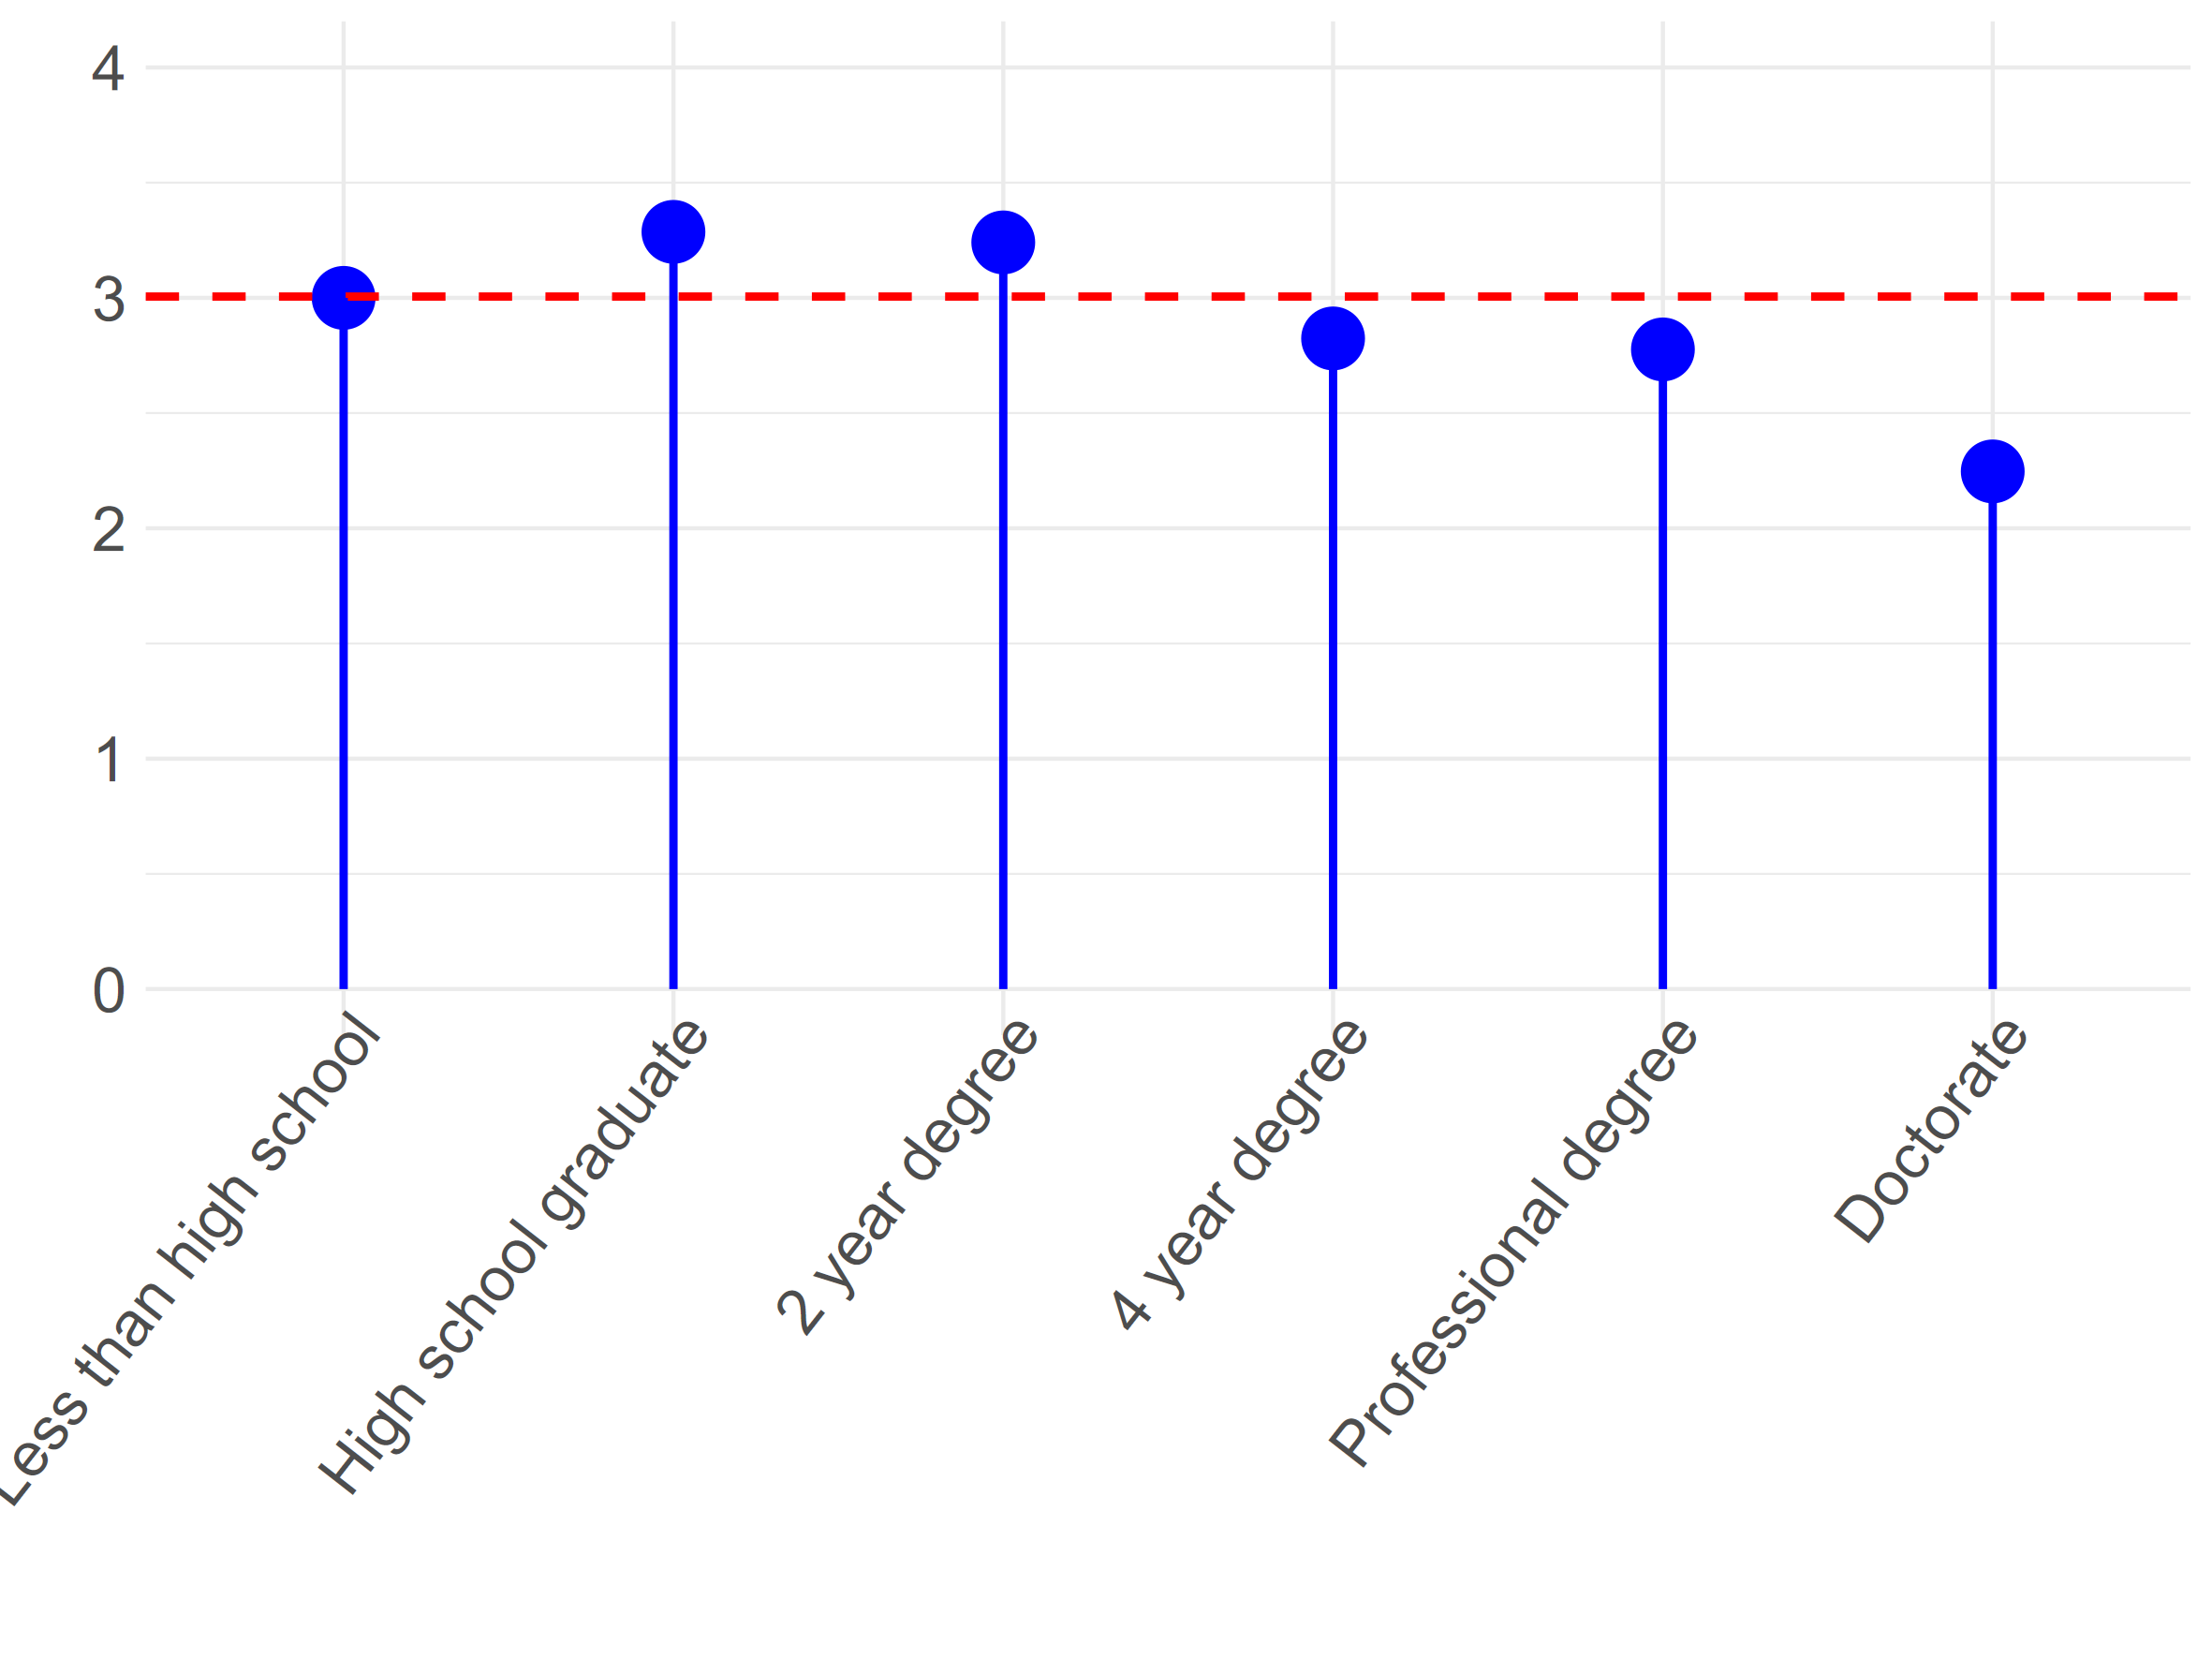
\includegraphics[width=1.0\textwidth]{Plots/uni-dist-grd-int-edu.png}
            \caption{Education}
            \label{fig:grd-int-edu}
    \end{subfigure}
     \begin{subfigure}[b]{0.3\textwidth}
        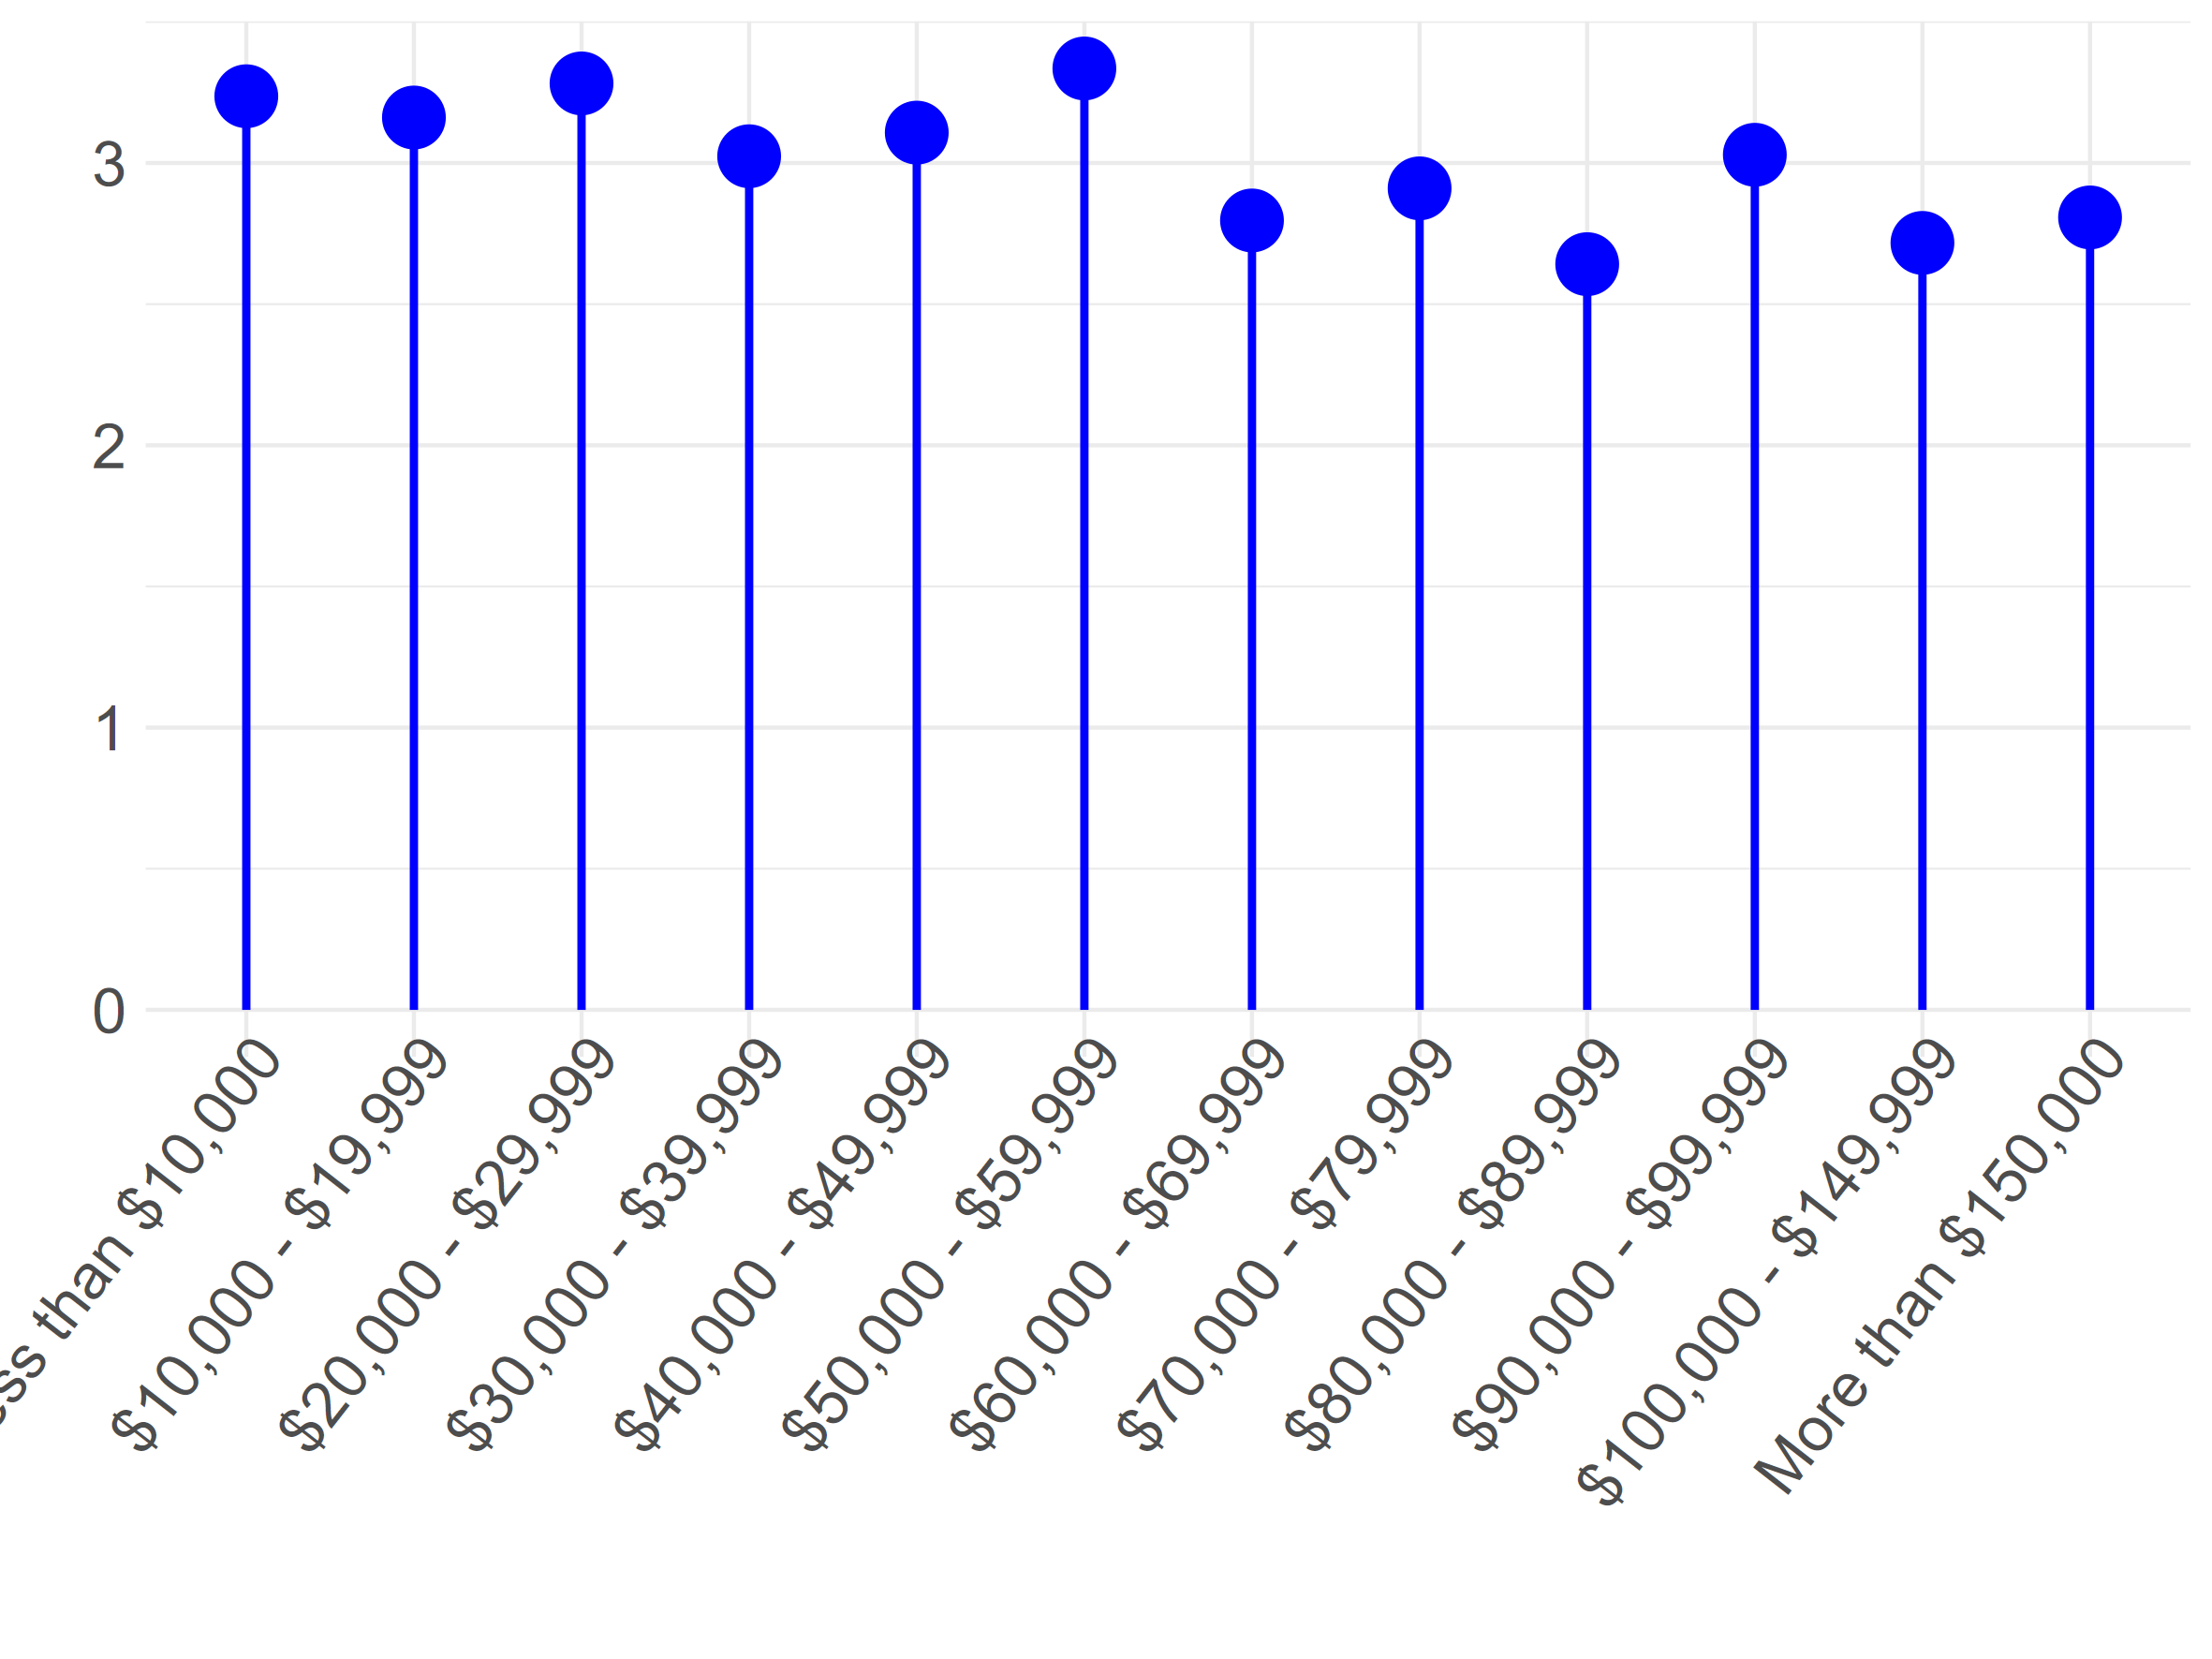
\includegraphics[width=1.0\textwidth]{Plots/uni-dist-grd-int-inc.png}
            \caption{Income}
            \label{fig:grd-int-inc}
    \end{subfigure}
     \begin{subfigure}[b]{0.3\textwidth}
        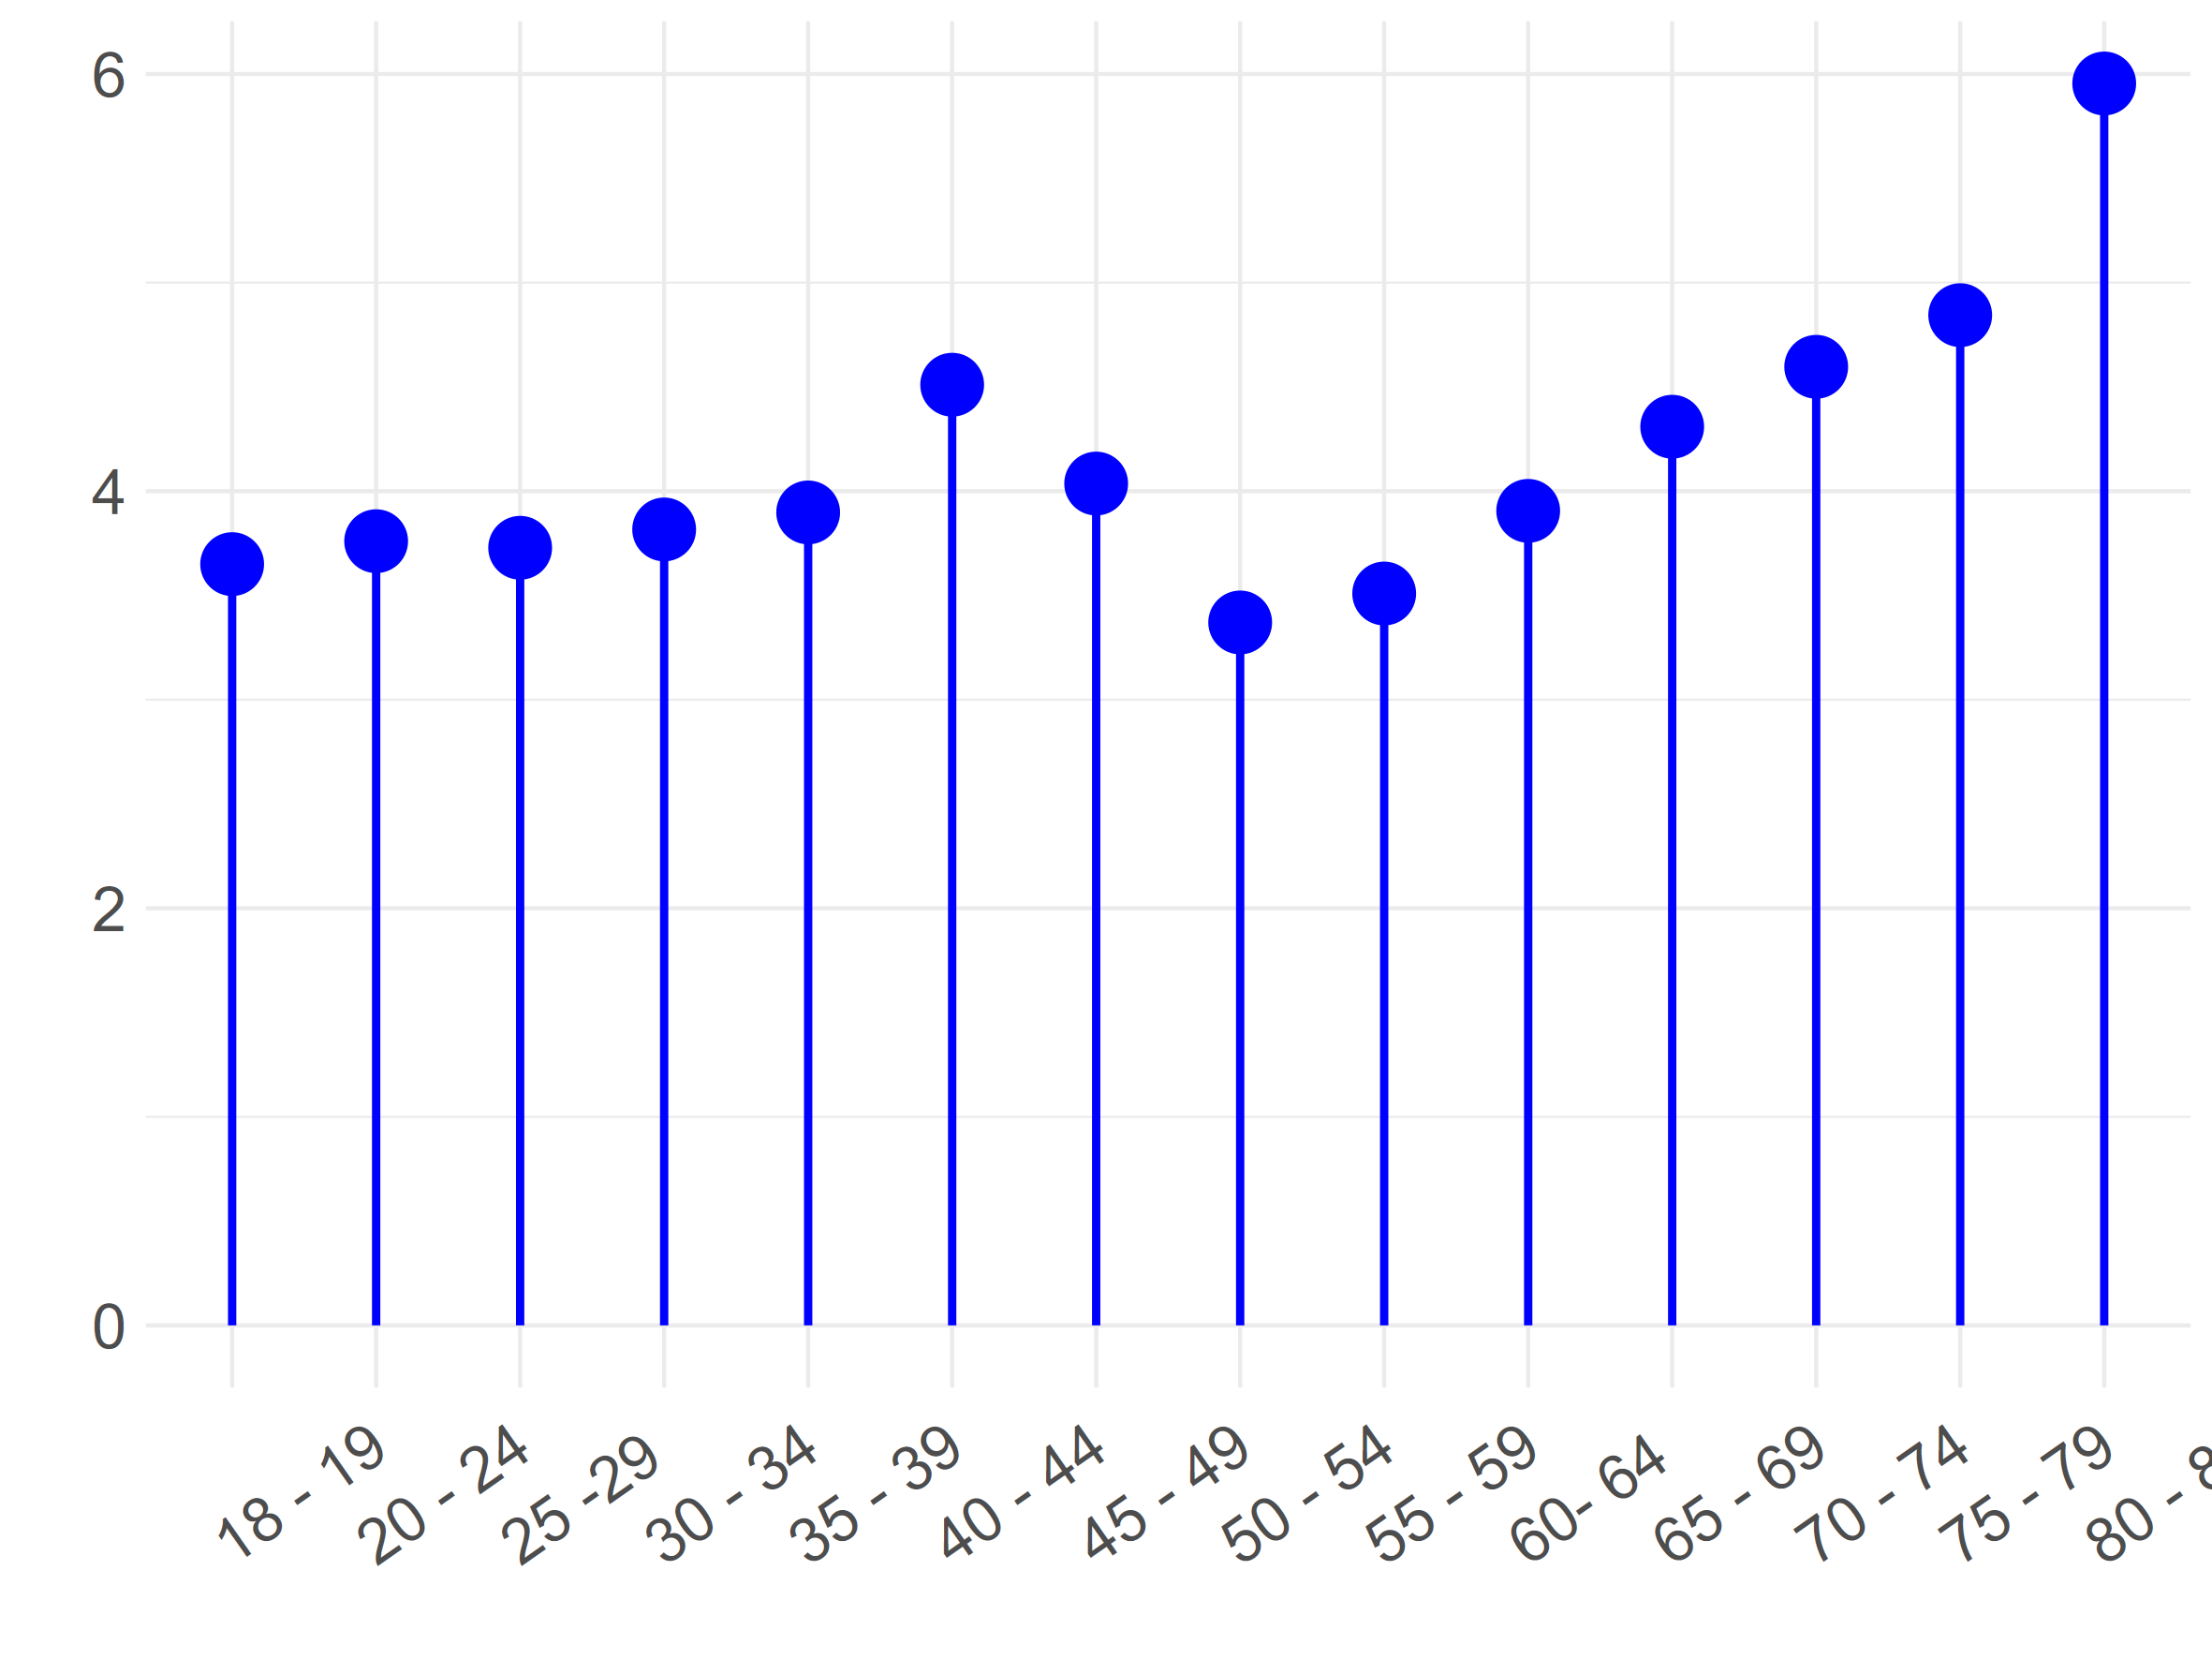
\includegraphics[width=1.0\textwidth]{Plots/uni-dist-grd-int-age.png}
            \caption{Age}
            \label{fig:grd-int-age}
    \end{subfigure}
     \begin{subfigure}[b]{0.3\textwidth}
        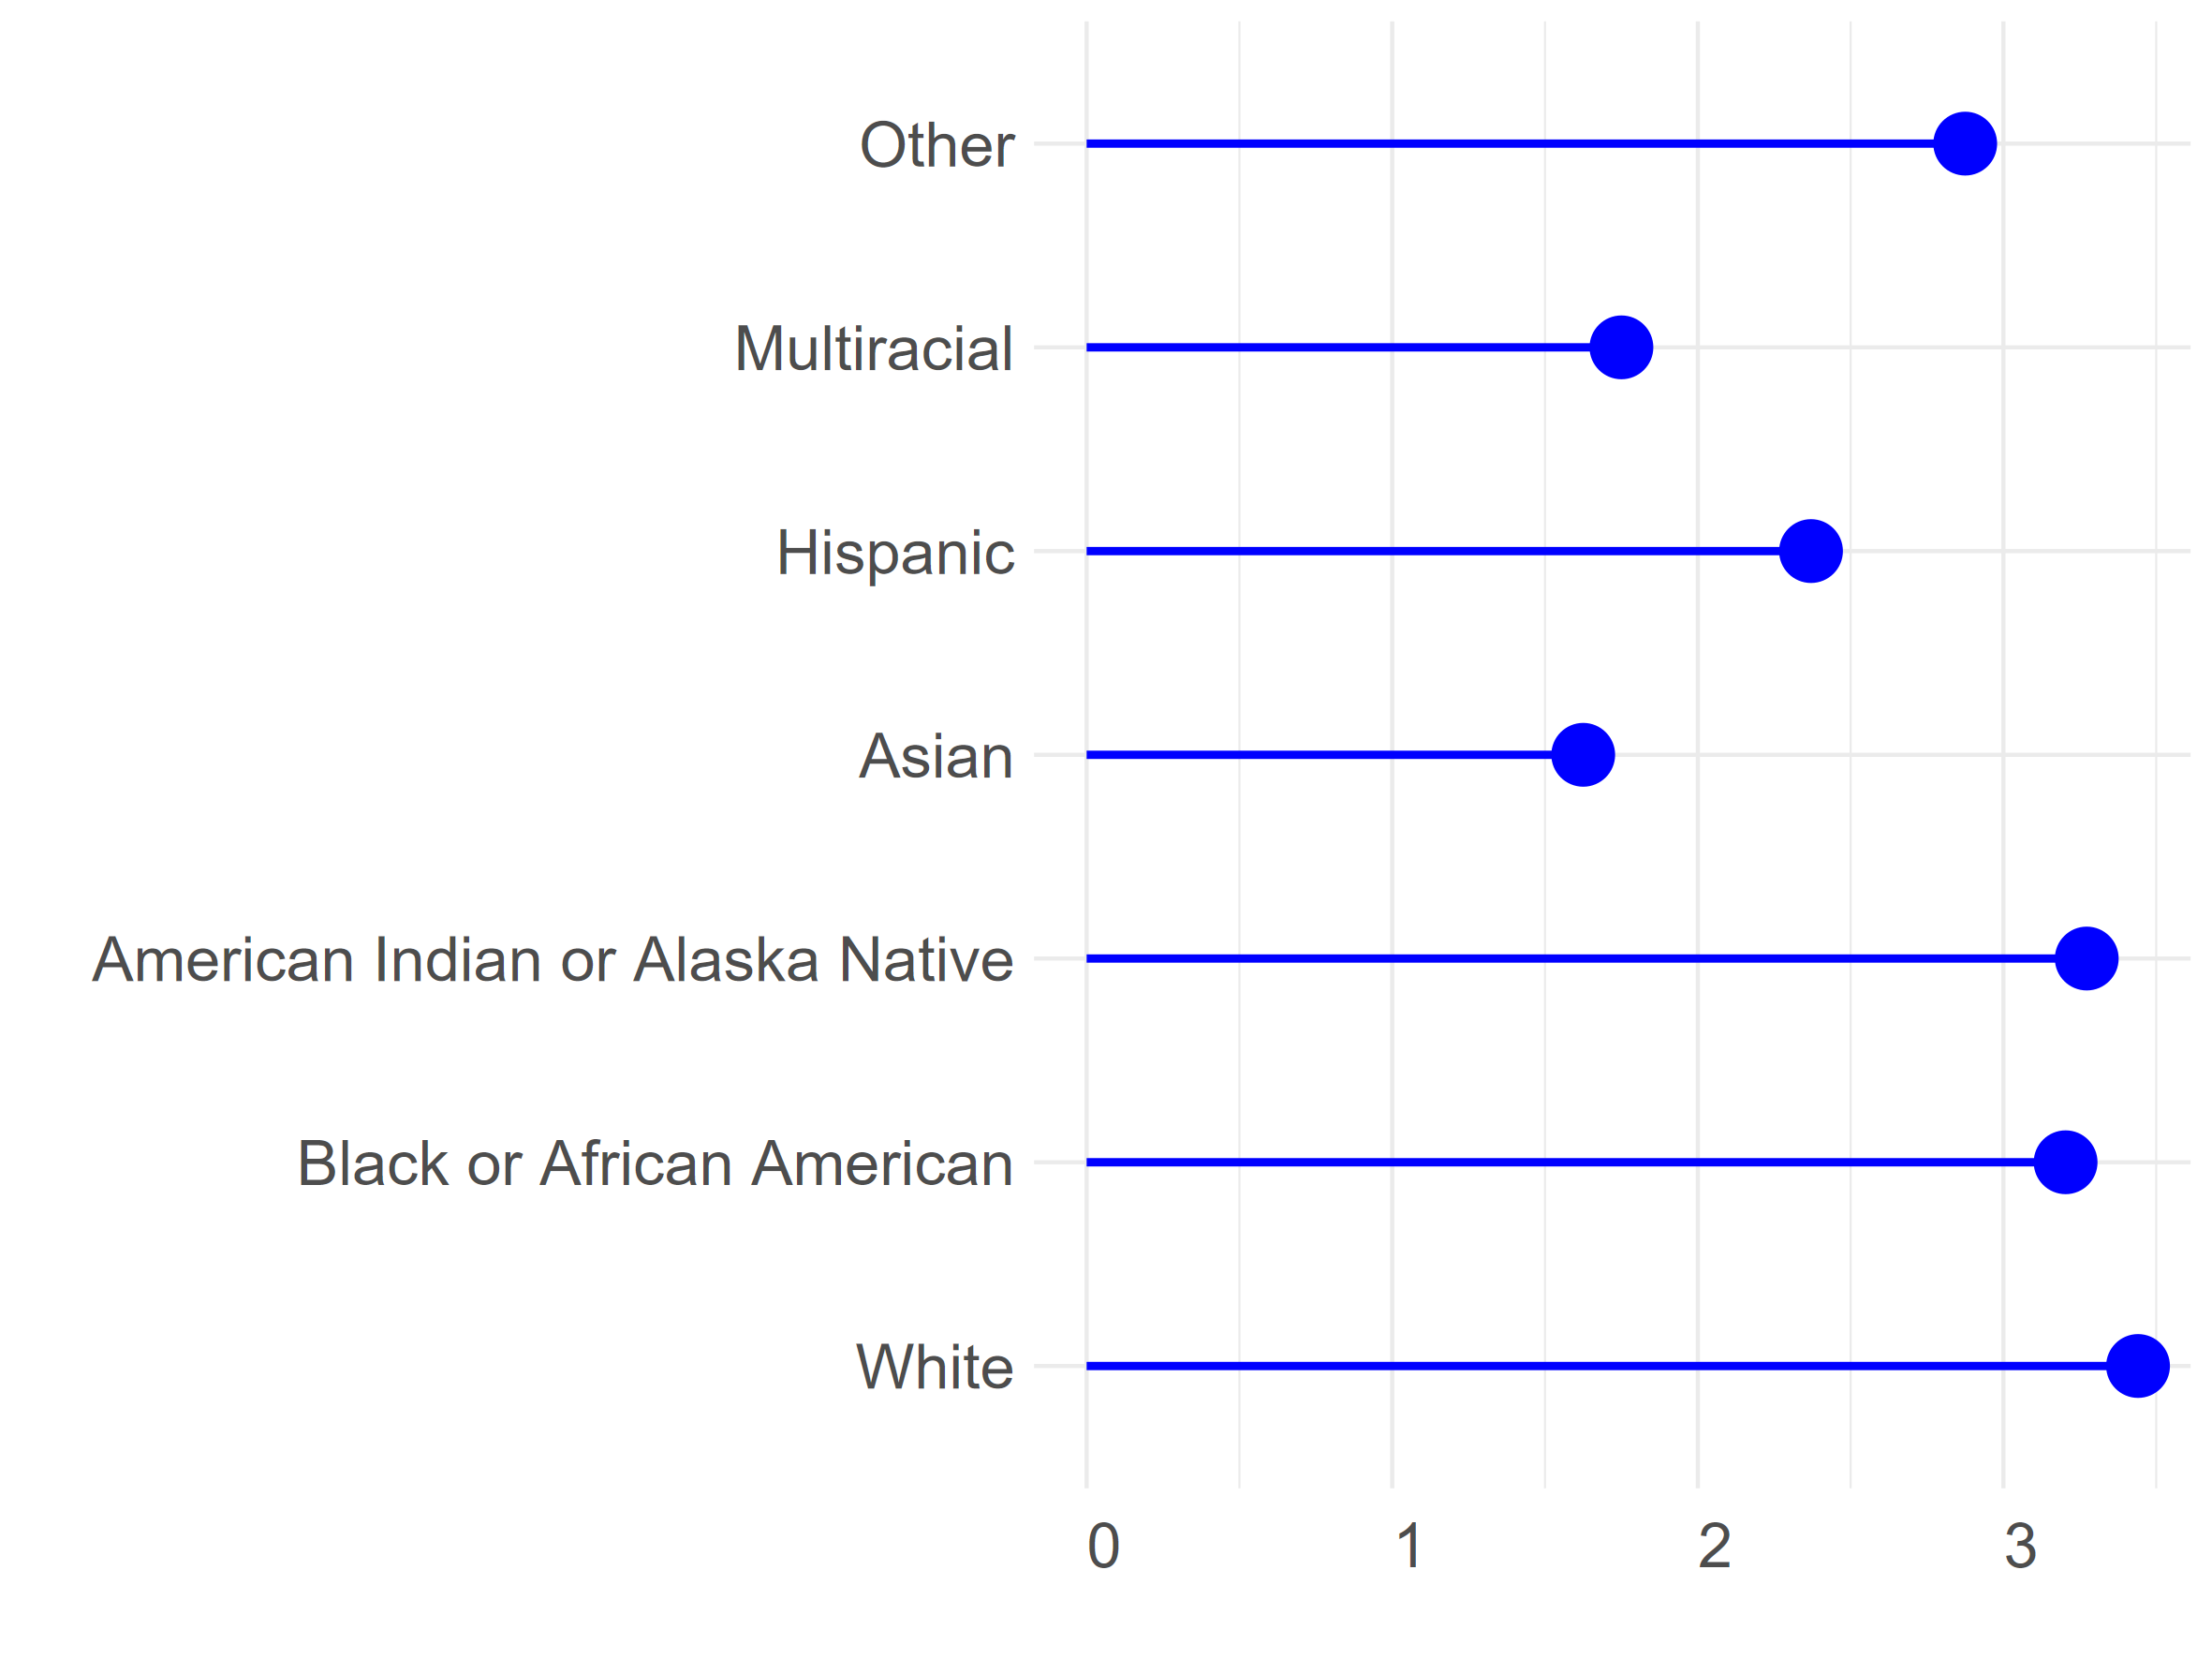
\includegraphics[width=1.0\textwidth]{Plots/uni-dist-grd-int-rac.png}
            \caption{Ethnoracial Identification}
            \label{fig:grd-int-rac}
    \end{subfigure}
     \begin{subfigure}[b]{0.3\textwidth}
        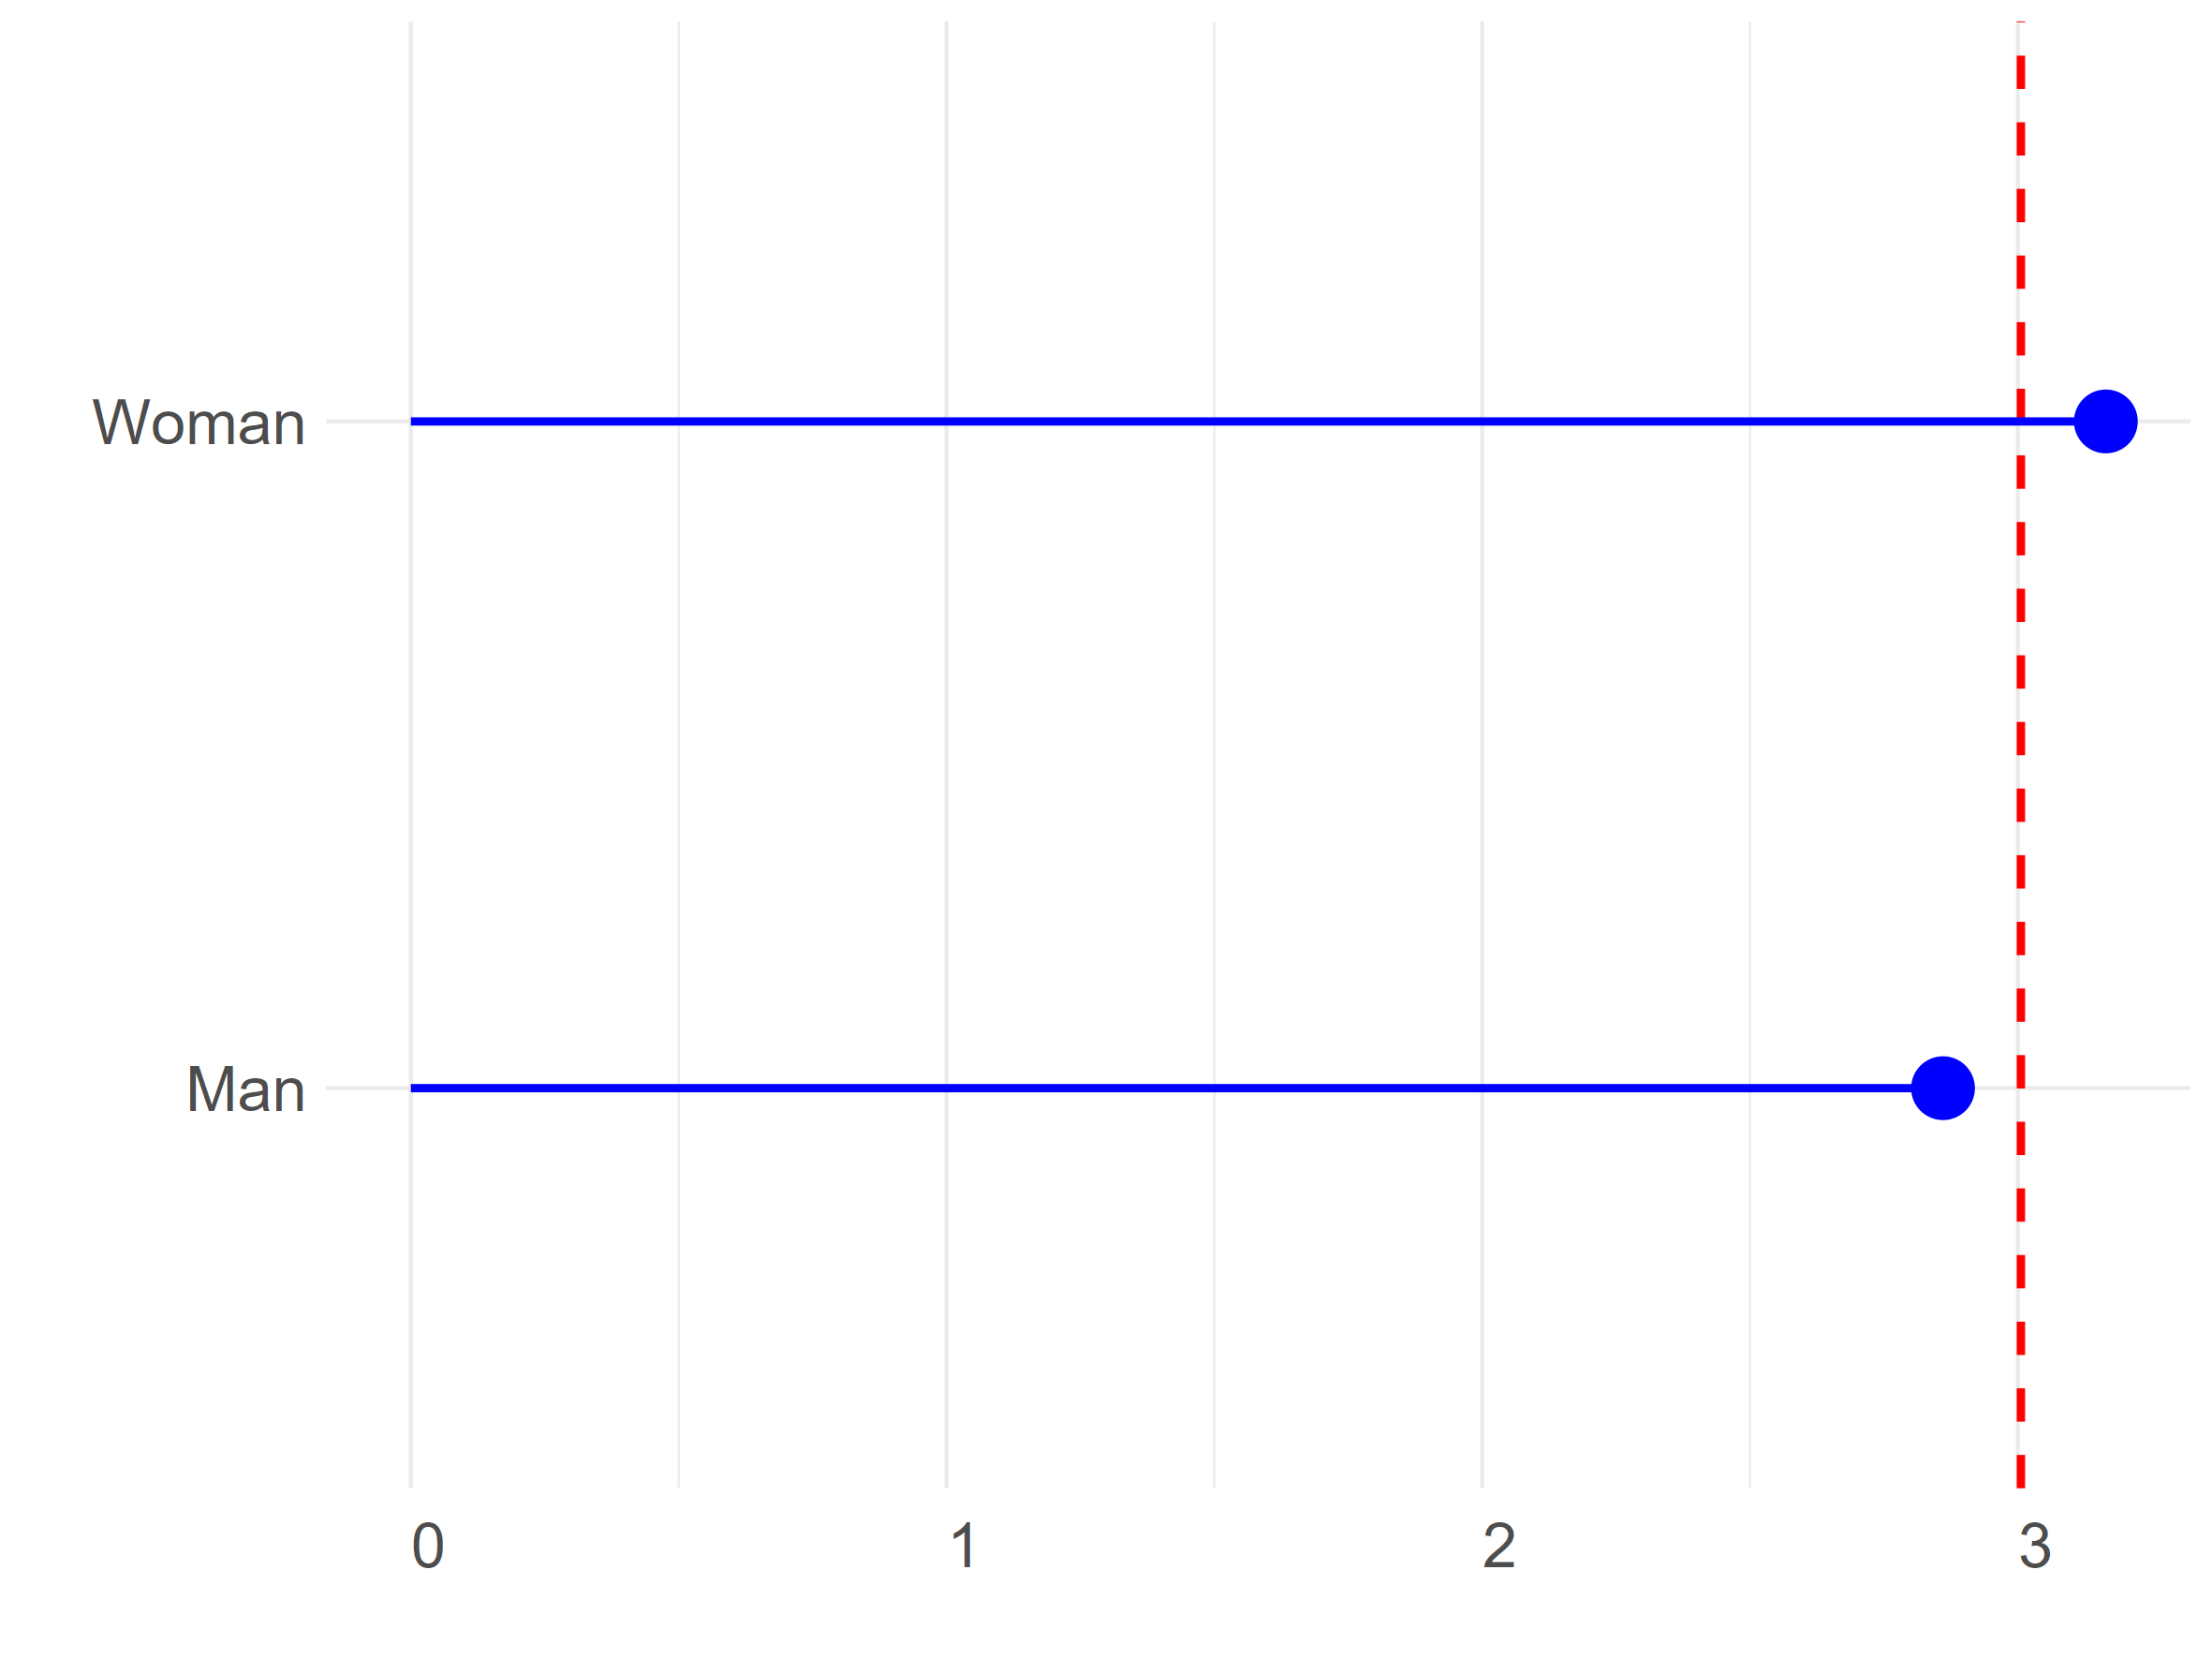
\includegraphics[width=1.0\textwidth]{Plots/uni-dist-grd-int-gen.png}
            \caption{Gender Identification}
            \label{fig:grd-int-gen}
    \end{subfigure}
    \caption{Average number of cultural dislikes across different socio-demographic characteristics.}
    \label{fig:grd-int}
\end{figure}
\newpage
\bibliography{references}
\bibliographystyle{apalike}

\end{document}
